\documentclass[12pt,letter]{article}
\usepackage{../downey_format}

\begin{document}
	
	% set the section number, along with figure and equation numbers
	\setcounter{section}{2}	
	\setcounter{figure}{0}   
	\renewcommand\thefigure{\thesection.\arabic{figure}}
	\setcounter{equation}{0}   
	\renewcommand\theequation{\thesection.\arabic{equation}}


\section{Machine Learning Workflows}

Machine learning workflows describe the sequence of steps used to transform raw engineering data into a trained and evaluated predictive model. Although the learning algorithm is important, successful machine learning applications often depend just as much on the quality of the data, the choice of features, and the way the model is evaluated. A well-organized workflow helps ensure that the model learns meaningful patterns rather than noise or accidental structure in the data.

Figure~\ref{fig:ml_workflow} illustrates a common machine learning workflow. The process begins by collecting data from experiments, sensors, simulations, or existing records. The data are then inspected and cleaned to identify missing values, outliers, inconsistent units, or other quality issues. After this preparation step, feature engineering is used to convert the raw data into informative inputs for the model. The model is then trained using a portion of the available data and tested using data that were not used during training.

\begin{figure}[h!]
	\centering
	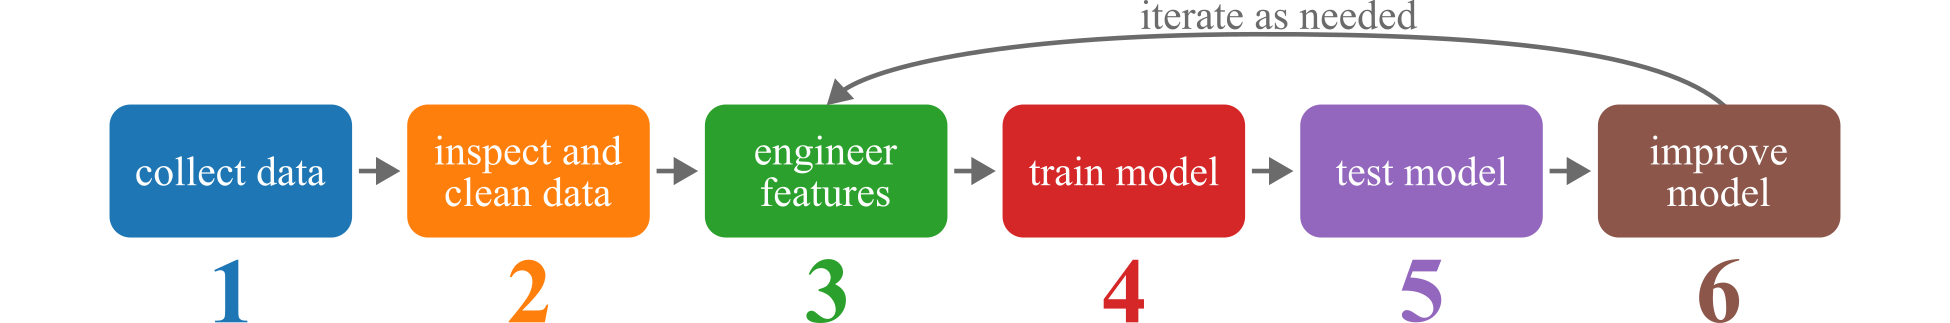
\includegraphics[width=6.5in]{../figures/ML_workflow}
	\caption{A typical machine learning workflow for engineering applications.}
	\label{fig:ml_workflow}
\end{figure}

The final step is improvement. If the model does not perform well enough, the workflow is repeated by revisiting earlier decisions. This may involve collecting more data, improving the data-cleaning process, changing the engineered features, tuning model parameters, or selecting a different learning algorithm. For this reason, machine learning should be viewed as an iterative process rather than a single pass through the data.

A typical workflow can be summarized as follows:

\begin{enumerate}
	\item \textbf{Collect data:} Gather measurements, simulations, experimental observations, or operational records.
	\item \textbf{Inspect and clean data:} Check the data for missing values, outliers, incorrect units, noise, and obvious errors.
	\item \textbf{Engineer features:} Transform the raw data into informative inputs that capture important patterns or physical behavior.
	\item \textbf{Train model:} Fit a machine learning model using the training data.
	\item \textbf{Test model:} Evaluate the trained model using data that were not used during training.
	\item \textbf{Improve model:} Refine the data, features, model settings, or learning algorithm based on the test results.
\end{enumerate}



\subsection{Feature Engineering}
\label{sec:feature_engineering}

Feature engineering is the process of transforming raw data into informative inputs that can be used by machine learning algorithms. Carefully designed features can significantly improve model performance and help capture important physical relationships in engineering data. 


Figure~\ref{fig:feature_engineering_roadmap} illustrates how raw engineering data can be transformed into a feature vector for machine learning. The features shown in this section are not the only features that can be extracted from data. Other useful inputs may include categorical features, countable features, indicator variables, domain-specific quantities, or features created from simulations and experiments. However, statistical, time-series, and frequency-domain features provide a useful starting point for building informative features from many engineering datasets.

\begin{figure}[h!]
	\centering
	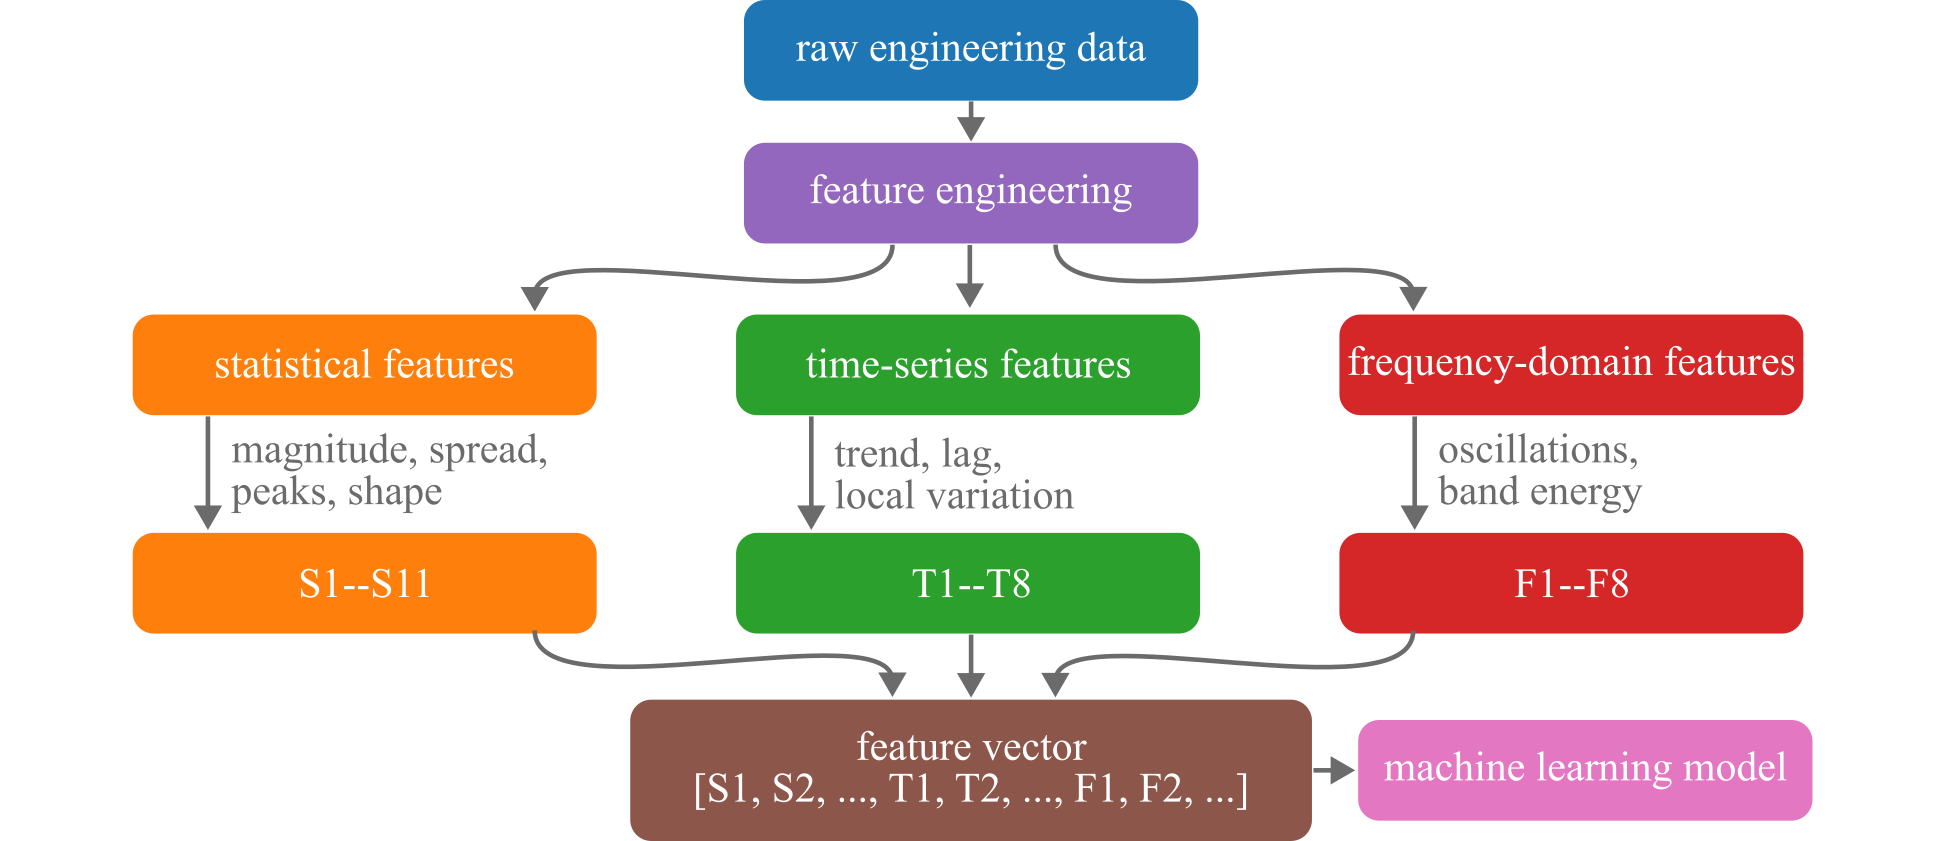
\includegraphics[width=6.5in]{../figures/feature_engineering}
	\caption{Feature engineering transforms raw engineering data into informative model inputs. Features may summarize the statistical properties, time-dependent behavior, or frequency content of the data.}
	\label{fig:feature_engineering_roadmap}
\end{figure}
\subsubsection{Statistical Features}

Statistical features summarize the distribution of values within a dataset, observation, or time window. These features are useful for describing the overall magnitude, variability, symmetry, and peak behavior of the data. Although statistical features are often computed from time-series measurements, they do not necessarily depend on the order of the samples in time.

Let \(x_i\) represent the \(i\)th value in a set of \(N\) measurements, let \(\bar{x}\) represent the mean value, and let \(s\) represent the sample standard deviation. Table~\ref{tab:statistical_features} lists a number of statistical features relevant in engineering. 

\begin{table}[H]
	\centering
	\caption{Common statistical features for engineering data.}
	\label{tab:statistical_features}
	\begin{tabular}{p{0.06\textwidth} p{0.22\textwidth} p{0.25\textwidth} p{0.37\textwidth}}
		\hline
		\textbf{No.} & \textbf{Feature} & \textbf{Equation} & \textbf{Physical Interpretation} \\
		\hline
		S1 & Maximum value 
		& \(\displaystyle \max(x_i)\) 
		& The maximum value captures the largest response in the signal. \\
		
		S2 & Minimum value 
		& \(\displaystyle \min(x_i)\) 
		& The minimum value captures the smallest response in the signal. \\
		
		S3 & Mean value 
		& \(\displaystyle \bar{x}=\frac{1}{N}\sum_{i=1}^{N}x_i\) 
		& The mean value describes the average level of the signal. \\
		
		S4 & Absolute mean value 
		& \(\displaystyle \frac{1}{N}\sum_{i=1}^{N}|x_i|\) 
		& The absolute mean value describes the average magnitude of the signal. \\
		
		S5 & Root mean square value 
		& \(\displaystyle x_{\mathrm{rms}}=\sqrt{\frac{1}{N}\sum_{i=1}^{N}x_i^2}\) 
		& The root mean square value describes the effective signal magnitude. \\
		
		S6 & Standard deviation 
		& \(\displaystyle s=\sqrt{\frac{1}{N-1}\sum_{i=1}^{N}(x_i-\bar{x})^2}\) 
		& The standard deviation describes how much the signal varies. \\
		
		S7 & Skewness 
		& \(\displaystyle \frac{1}{N}\sum_{i=1}^{N}\left(\frac{x_i-\bar{x}}{s}\right)^3\) 
		& Skewness describes whether the signal is biased toward one side. \\
		
		S8 & Kurtosis 
		& \(\displaystyle \frac{1}{N}\sum_{i=1}^{N}\left(\frac{x_i-\bar{x}}{s}\right)^4\) 
		& Kurtosis describes whether the signal contains sharp peaks or outliers. \\
		
		S9 & Shape factor 
		& \(\displaystyle \frac{x_{\mathrm{rms}}}{\frac{1}{N}\sum_{i=1}^{N}|x_i|}\) 
		& The shape factor compares the effective magnitude to the average magnitude. \\
		
		S10 & Crest factor 
		& \(\displaystyle \frac{\max(|x_i|)}{x_{\mathrm{rms}}}\) 
		& The crest factor compares the largest peak to the effective signal level. \\
		
		S11 & Impulse factor 
		& \(\displaystyle \frac{\max(|x_i|)}{\frac{1}{N}\sum_{i=1}^{N}|x_i|}\) 
		& The impulse factor compares the largest peak to the average magnitude. \\
		\hline
	\end{tabular}
\end{table}


\subsubsection{Time-Series Features}

Time-series features describe how a signal changes with time. Unlike statistical features, these features depend on the order of the samples. They are useful when the timing, trend, persistence, or local variation of the signal contains important information.

Table~\ref{tab:time_series_features} lists a number of time-series features relevant in engineering. Let \(x_i\) represent the signal value at time index \(i\), let \(\Delta t\) represent the sampling interval, let \(k\) represent a lag, and let \(w\) represent the number of samples in a moving window. The local mean over a window is denoted as \(\bar{x}_{i,w}\).



\begin{table}[H]
	\centering
	\caption{Common time-series features for engineering data.}
	\label{tab:time_series_features}
	\begin{tabular}{p{0.05\textwidth} p{0.25\textwidth} p{0.30\textwidth} p{0.30\textwidth}}
		\hline
		\textbf{No.} & \textbf{Feature} & \textbf{Equation} & \textbf{Physical Interpretation} \\
		\hline
		T1 & Lagged value 
		& \(\displaystyle x_{i-k}\) 
		& A lagged value captures the recent history of the signal. \\
		
		T2 & First difference 
		& \(\displaystyle x_i-x_{i-1}\) 
		& The first difference captures the step-to-step change in the signal. \\
		
		T3 & Rate of change 
		& \(\displaystyle \frac{x_i-x_{i-1}}{\Delta t}\) 
		& The rate of change describes how quickly the signal changes with time. \\
		
		T4 & Moving average 
		& \(\displaystyle \frac{1}{w}\sum_{j=i-w+1}^{i}x_j\) 
		& The moving average captures the local trend of the signal. \\
		
		T5 & Rolling standard deviation 
		& \(\displaystyle \sqrt{\frac{1}{w-1}\sum_{j=i-w+1}^{i}(x_j-\bar{x}_{i,w})^2}\) 
		& The rolling standard deviation captures local variability. \\
		
		T6 & Rolling maximum 
		& \(\displaystyle \max(x_{i-w+1},\ldots,x_i)\) 
		& The rolling maximum captures recent peak behavior. \\
		
		T7 & Rolling minimum 
		& \(\displaystyle \min(x_{i-w+1},\ldots,x_i)\) 
		& The rolling minimum captures recent low-response behavior. \\
		
		T8 & Zero-crossing rate 
		& \(\displaystyle \frac{1}{w-1}\sum_{j=i-w+2}^{i}\mathbb{I}(x_jx_{j-1}<0)\) 
		& The zero-crossing rate captures how often the signal changes sign \protect\footnotemark[1]. \\
		\hline
	\end{tabular}
\end{table}




\footnotetext[1]{\(\mathbb{I}(\cdot)\) is an indicator function that equals 1 when the condition is true and 0 otherwise.}



\subsubsection{Frequency-Domain Features}

Frequency-domain features describe how the content of a signal is distributed across frequency. These features are commonly extracted by applying a Fourier transform to a measured signal and then summarizing the resulting spectrum. Table~\ref{tab:frequency_domain_features} lists a number of frequency-domain features relevant in engineering. They are useful when the important behavior in the data is related to oscillations, repeating patterns, or changes in the balance between slow and rapid variations. 

Let \(P(f)\) represent the power spectrum of the signal at frequency \(f\), and let \(B_L\), \(B_M\), and \(B_H\) represent the low-, middle-, and high-frequency bands. The total spectral energy is defined as
\begin{equation}
E_{\mathrm{total}} = \int P(f)\,df .
\end{equation}
In a specific engineering application, the frequency bands should be selected based on the system being studied. When no application-specific bands are known, the usable frequency range can be divided into low-, middle-, and high-frequency regions as a starting point.

\begin{table}[H]
	\centering
	\caption{Common frequency-domain features for engineering time-series data.}
	\label{tab:frequency_domain_features}
	\begin{tabular}{p{0.06\textwidth} p{0.22\textwidth} p{0.25\textwidth} p{0.37\textwidth}}
		\hline
		\textbf{No.} & \textbf{Feature} & \textbf{Equation} & \textbf{Physical Interpretation} \\
		\hline
		F1 & Dominant frequency 
		& \(\displaystyle f_{\mathrm{dom}}=\arg\max_f P(f)\) 
		& The dominant frequency captures the strongest periodic behavior. \\
		
		F2 & Spectral centroid 
		& \(\displaystyle f_c=\frac{\int fP(f)\,df}{\int P(f)\,df}\) 
		& The spectral centroid describes where the spectrum is centered. \\
		
		F3 & Spectral bandwidth 
		& \(\displaystyle \sqrt{\frac{\int (f-f_c)^2P(f)\,df}{\int P(f)\,df}}\) 
		& The spectral bandwidth describes how widely the energy is spread. \\
		
		F4 & Low-frequency energy ratio 
		& \(\displaystyle \frac{\int_{B_\text{L}}P(f)\,df}{E_{\mathrm{total}}}\) 
		& The low-frequency energy ratio measures the share of energy in slow behavior. \\
		
		F5 & Middle-frequency energy ratio 
		& \(\displaystyle \frac{\int_{B_\text{M}}P(f)\,df}{E_{\mathrm{total}}}\) 
		& The middle-frequency energy ratio measures the share of energy in mid-range behavior. \\
		
		F6 & High-frequency energy ratio 
		& \(\displaystyle \frac{\int_{B_\text{H}}P(f)\,df}{E_{\mathrm{total}}}\) 
		& The high-frequency energy ratio measures the share of energy in rapid behavior. \\
		
		F7 & High-to-low frequency energy ratio 
		& \(\displaystyle \frac{\int_{B_\text{H}}P(f)\,df}{\int_{B_\text{L}}P(f)\,df}\) 
		& The high-to-low frequency energy ratio compares rapid behavior to slow behavior. \\
		
		F8 & Peak-to-total spectral energy ratio 
		& \(\displaystyle \frac{P(f_{\mathrm{dom}})}{E_{\mathrm{total}}}\) 
		& The peak-to-total spectral energy ratio measures how dominant the largest frequency peak is. \\
		\hline
	\end{tabular}
\end{table}




\pagebreak

\subsection{Training and Testing Data}

Training a predictive model on a dataset and then testing it with the same data is a fundamental error in methodology. Such a model could simply memorize the labels of the training samples, achieving perfect performance during training but failing to make any useful predictions on new, unseen data. This phenomenon is known as overfitting. To prevent this, it is standard practice in supervised machine learning to reserve a portion of the available data as a test set, denoted as $\textbf{X}_\text{test}$ and $\textbf{y}_\text{test}$.

		\begin{figure}[H]
			\centering
			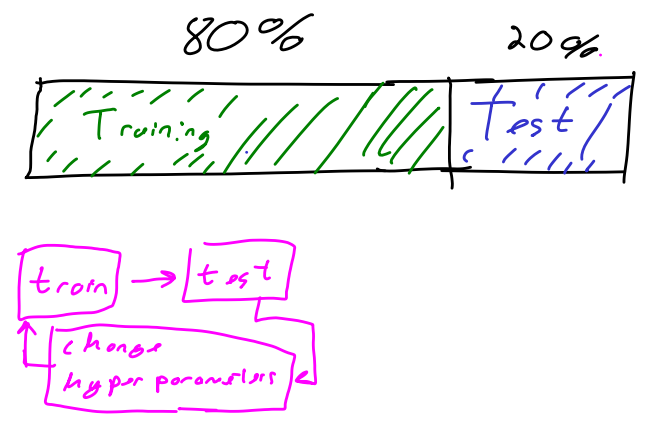
\includegraphics[]{../figures/training_test_datasets}
			\caption{Splitting data up into training and testing subsets.}
			\label{fig:training_test_datasets}
		\end{figure}


		\begin{figure}[H]
			\centering
			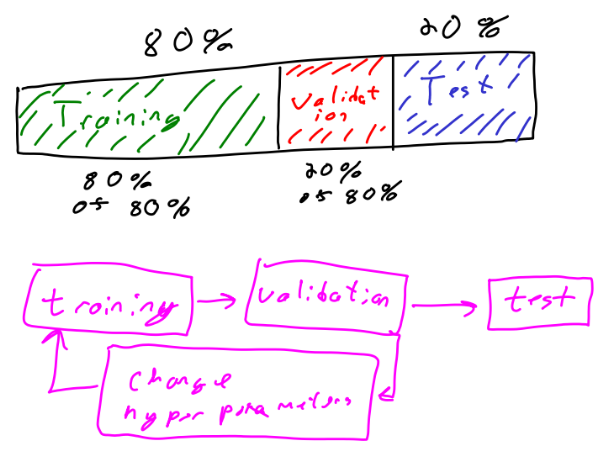
\includegraphics[]{../figures/training_validation_test_datasets}
			\caption{Splitting data up into training, validation, and testing subsets.}
			\label{fig:training_validation_test_datasets}
		\end{figure}


The function \texttt{sklearn.model\_selection.train\_test\_split} in scikit-learn randomly divides arrays or matrices into training and testing subsets.


\subsection{Pipelines}


Pipelines in scikit-learn streamline the process by sequentially applying a list of transformations followed by a final estimator to a dataset. Employing pipelines allows for the integration of multiple processing steps, which can then be cross-validated together while experimenting with various parameters. Fig.~\ref{fig:AutoML_diagram} illustrates a typical pipeline configuration in scikit-learn.



		\begin{figure}[H]
			\centering
			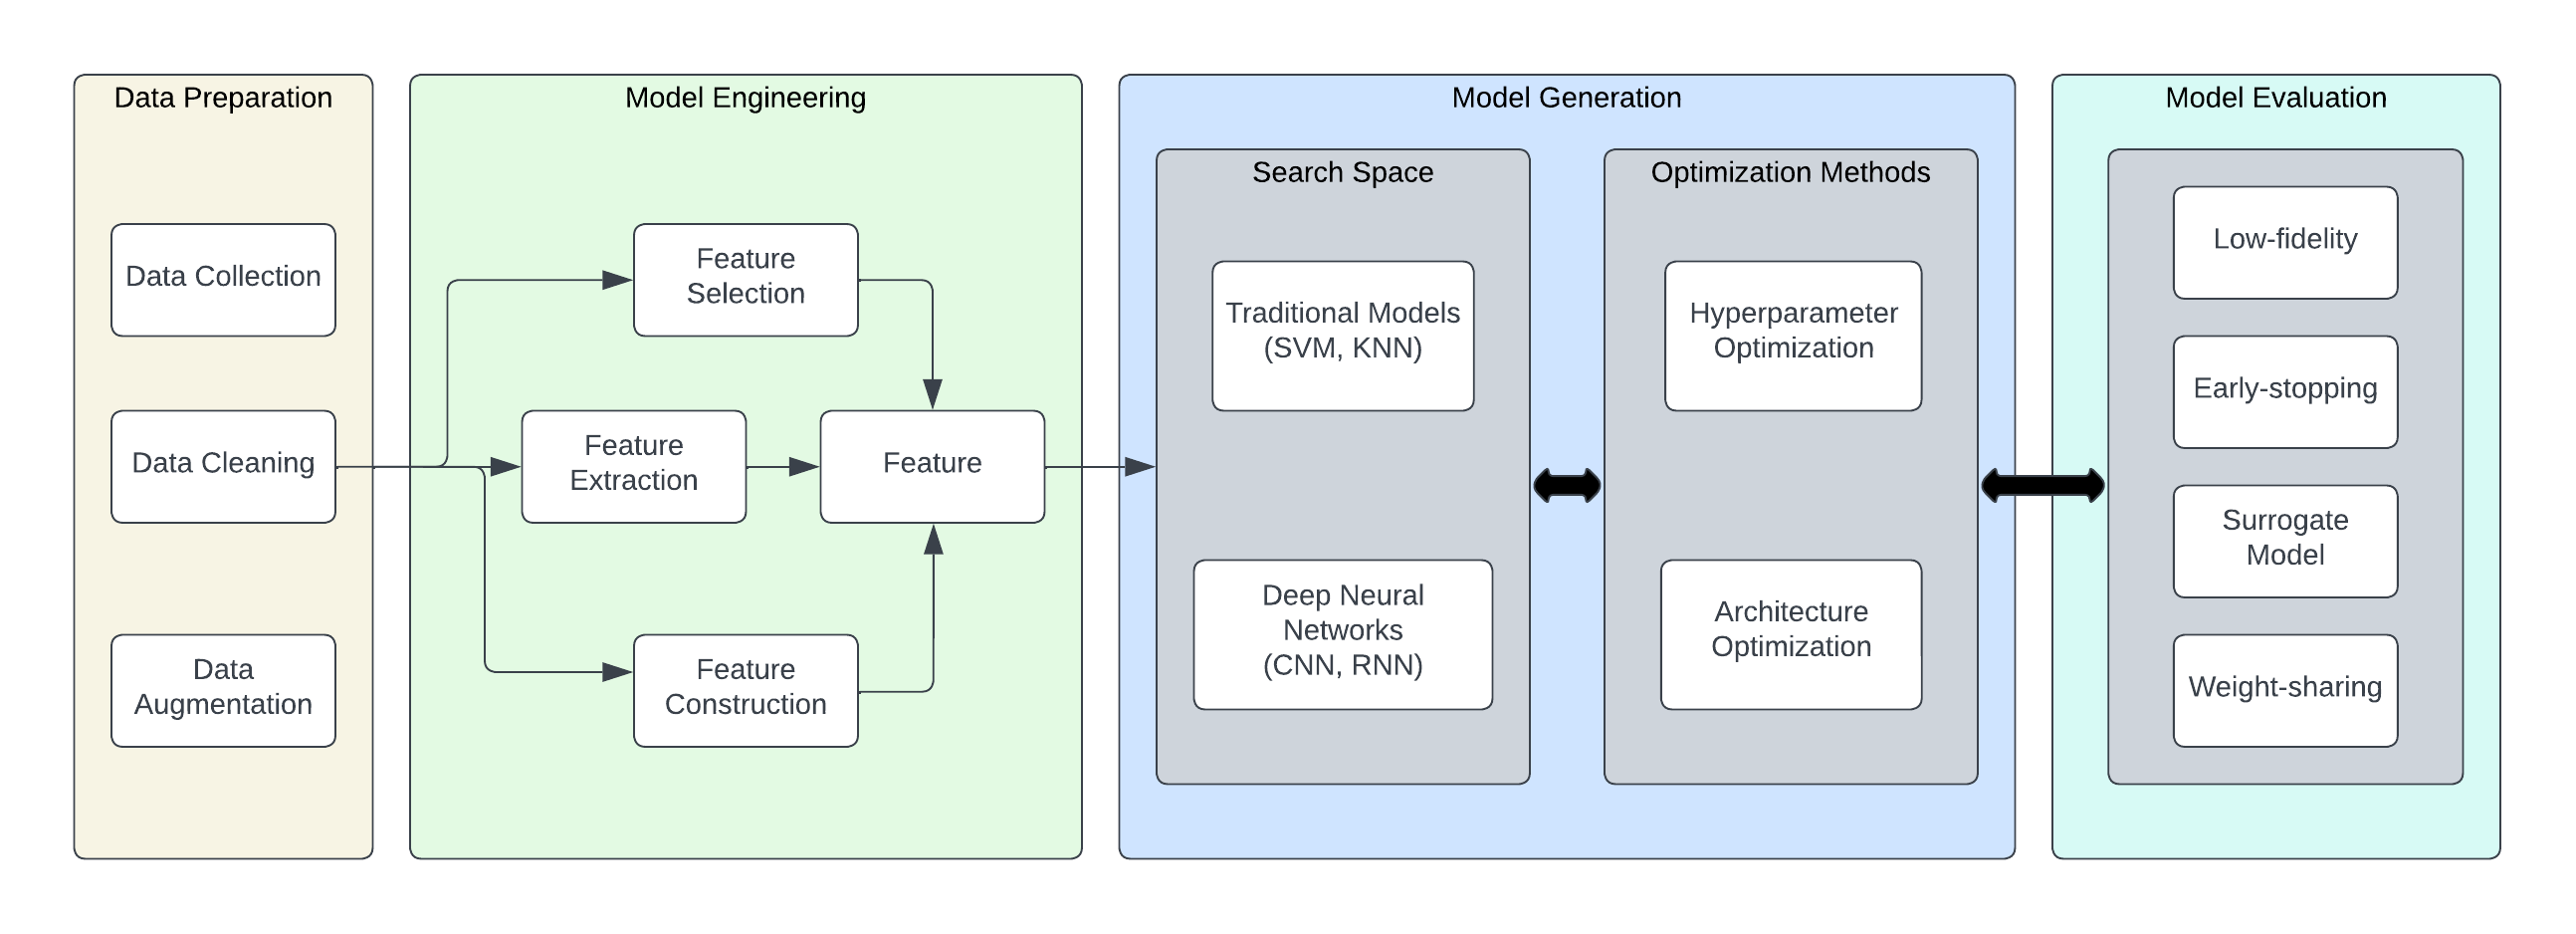
\includegraphics[width=6.5in]{../figures/AutoML_diagram}
			\caption{Pipeline setup for the automated deployment of pre-processing and modeling steps.\protect\footnotemark[1]}
			\label{fig:AutoML_diagram}
		\end{figure}


\footnotetext[1]{Modified from PopovaZhuhadar, CC BY-SA 4.0 $<$https://creativecommons.org/licenses/by-sa/4.0$>$, via Wikimedia Commons}

\subsection{Learning Curves}

Performing Polynomial Regression with a high degree typically allows for a closer fit to the training data compared to simple Linear Regression. For instance, Figure~\ref{fig:overfitting_1} demonstrates the application of a 30-degree polynomial model to a set of training data, contrasting it with both a linear model and a quadratic model (2\textsuperscript{nd}-degree polynomial). Observe how the 30-degree polynomial model contorts to closely match the training instances.
\begin{itemize}
\item The linear model exhibits underfitting.
\item The high-degree Polynomial Regression model drastically overfits the training data.
\item Among these, the quadratic model is likely to generalize best.
\end{itemize}
In this instance, the appropriateness of the quadratic model is clear since the data was initially generated using such a model. However, in real-world scenarios where the underlying function of the data is unknown, determining the optimal complexity for your model can be challenging. How can you ascertain whether your model is overfitting or underfitting the data?

\begin{figure}[h]
\centering
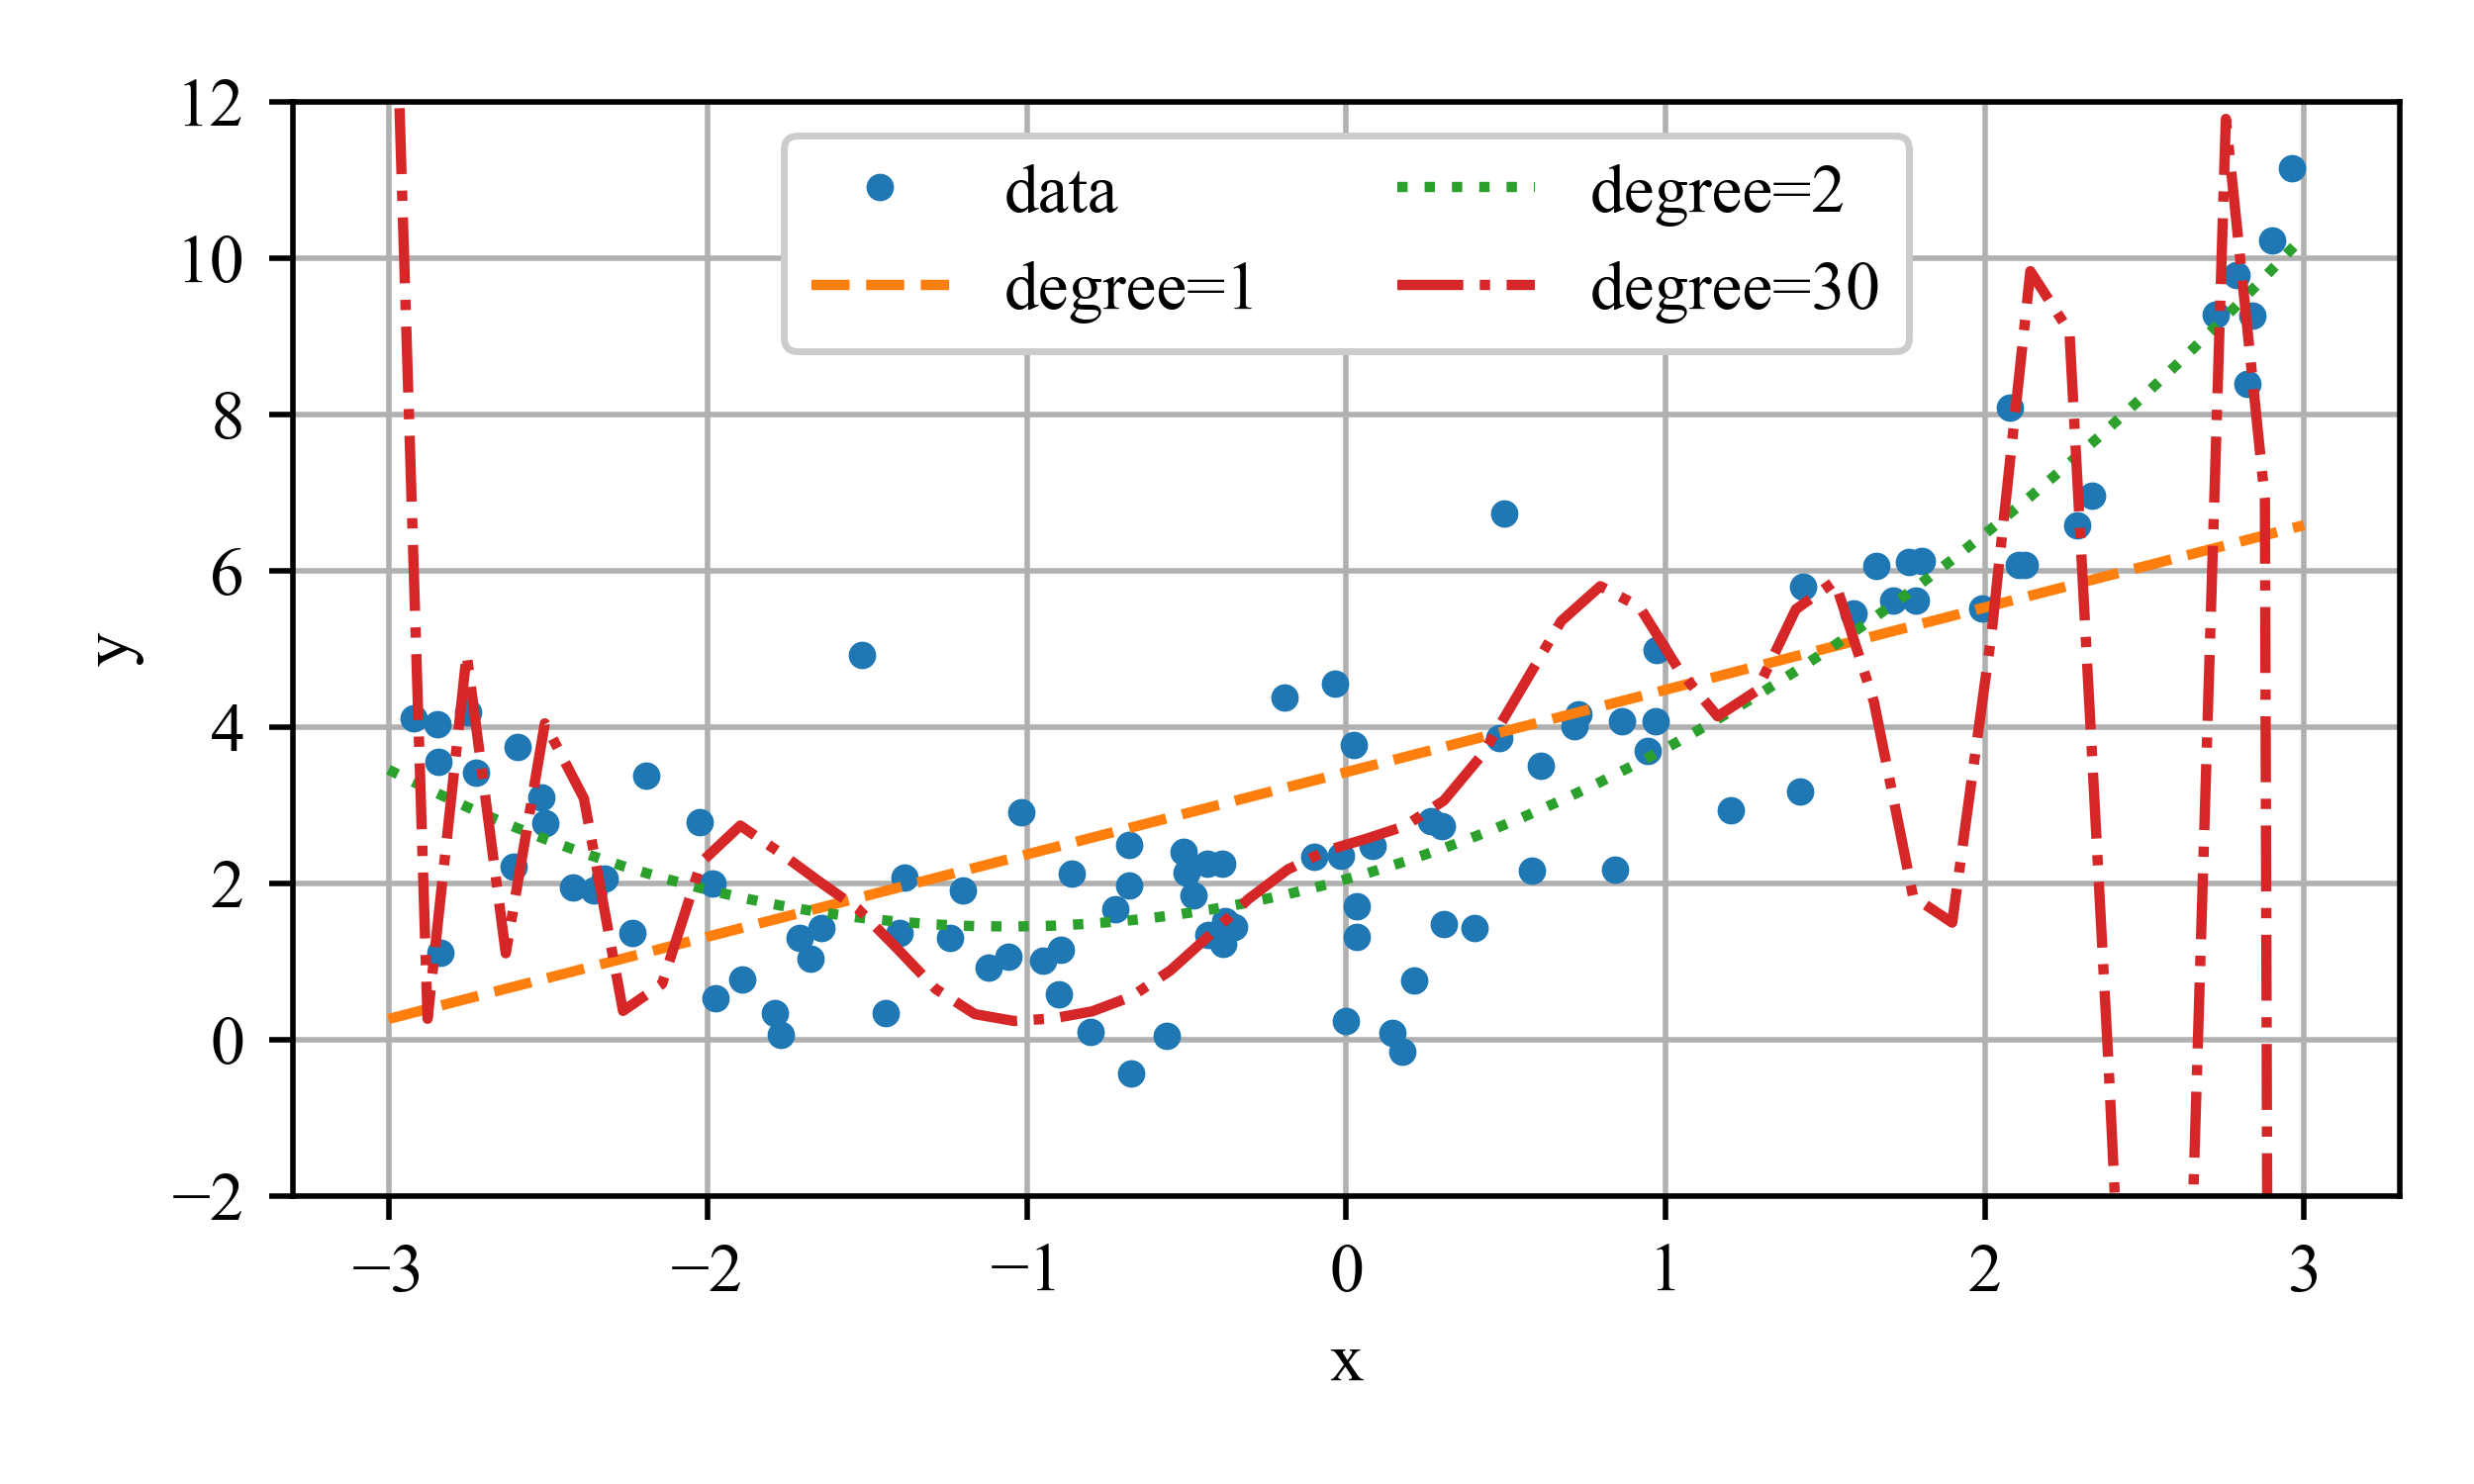
\includegraphics[]{../figures/overfitting_1.png}
\caption{Polynomial regression showing underfitting (degree=1), a respectable model fit (degree=2), and overfitting (degree=30).}
\label{fig:overfitting_1}
\end{figure}





\begin{figure}[H]
\centering
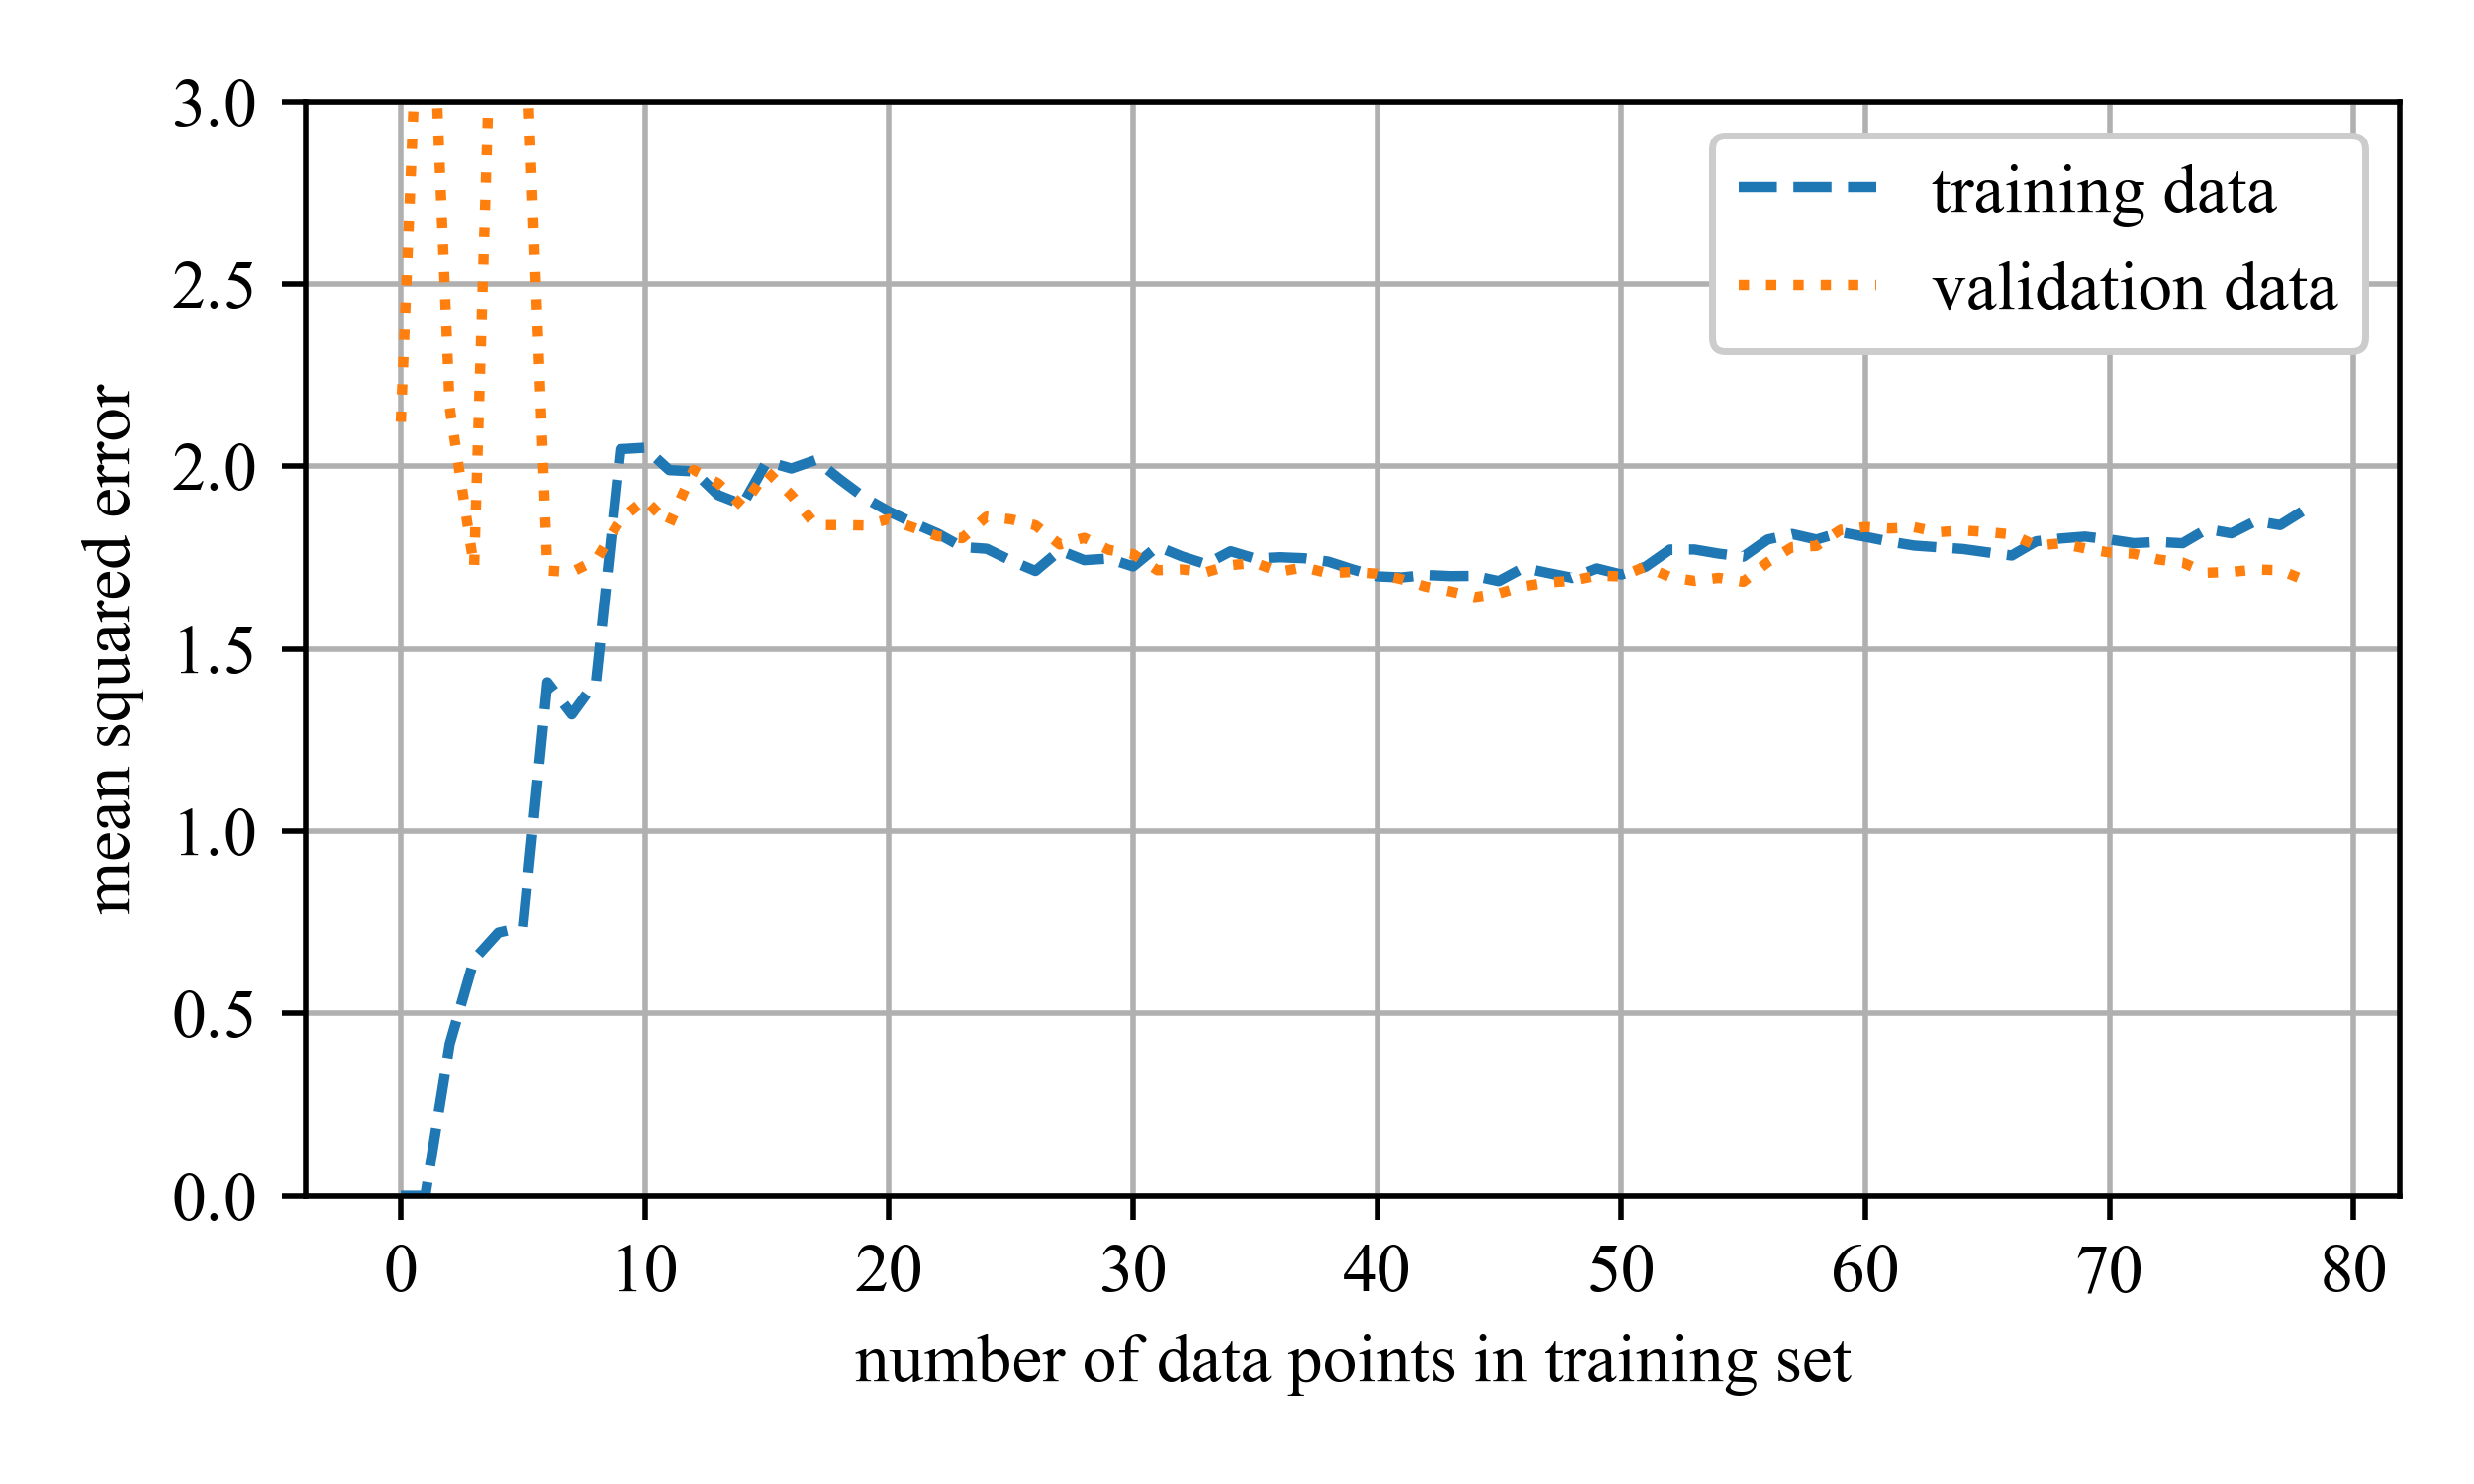
\includegraphics[]{../figures/overfitting_2.png}
\caption{Learning curves for the underfitting linear model (degree=1) where underfitting is evident because both curves have plateaued; they are close together and relatively high.}
\label{fig:overfitting_2}
\end{figure}

Examining the model's behavior in figures~\ref{fig:overfitting_2}~and~~\ref{fig:overfitting_3} on the training set shows a clear trend. With only one or two samples the fit is perfect, so the error curve begins at zero. As additional observations are introduced the model can no longer capture every point exactly, partly because of measurement noise and partly because the underlying relationship is nonlinear, and consequently the training error rises. After a sufficient number of samples the curve flattens out; beyond this plateau adding further data neither markedly lowers nor raises the average error.

\begin{figure}[H]
    \centering
    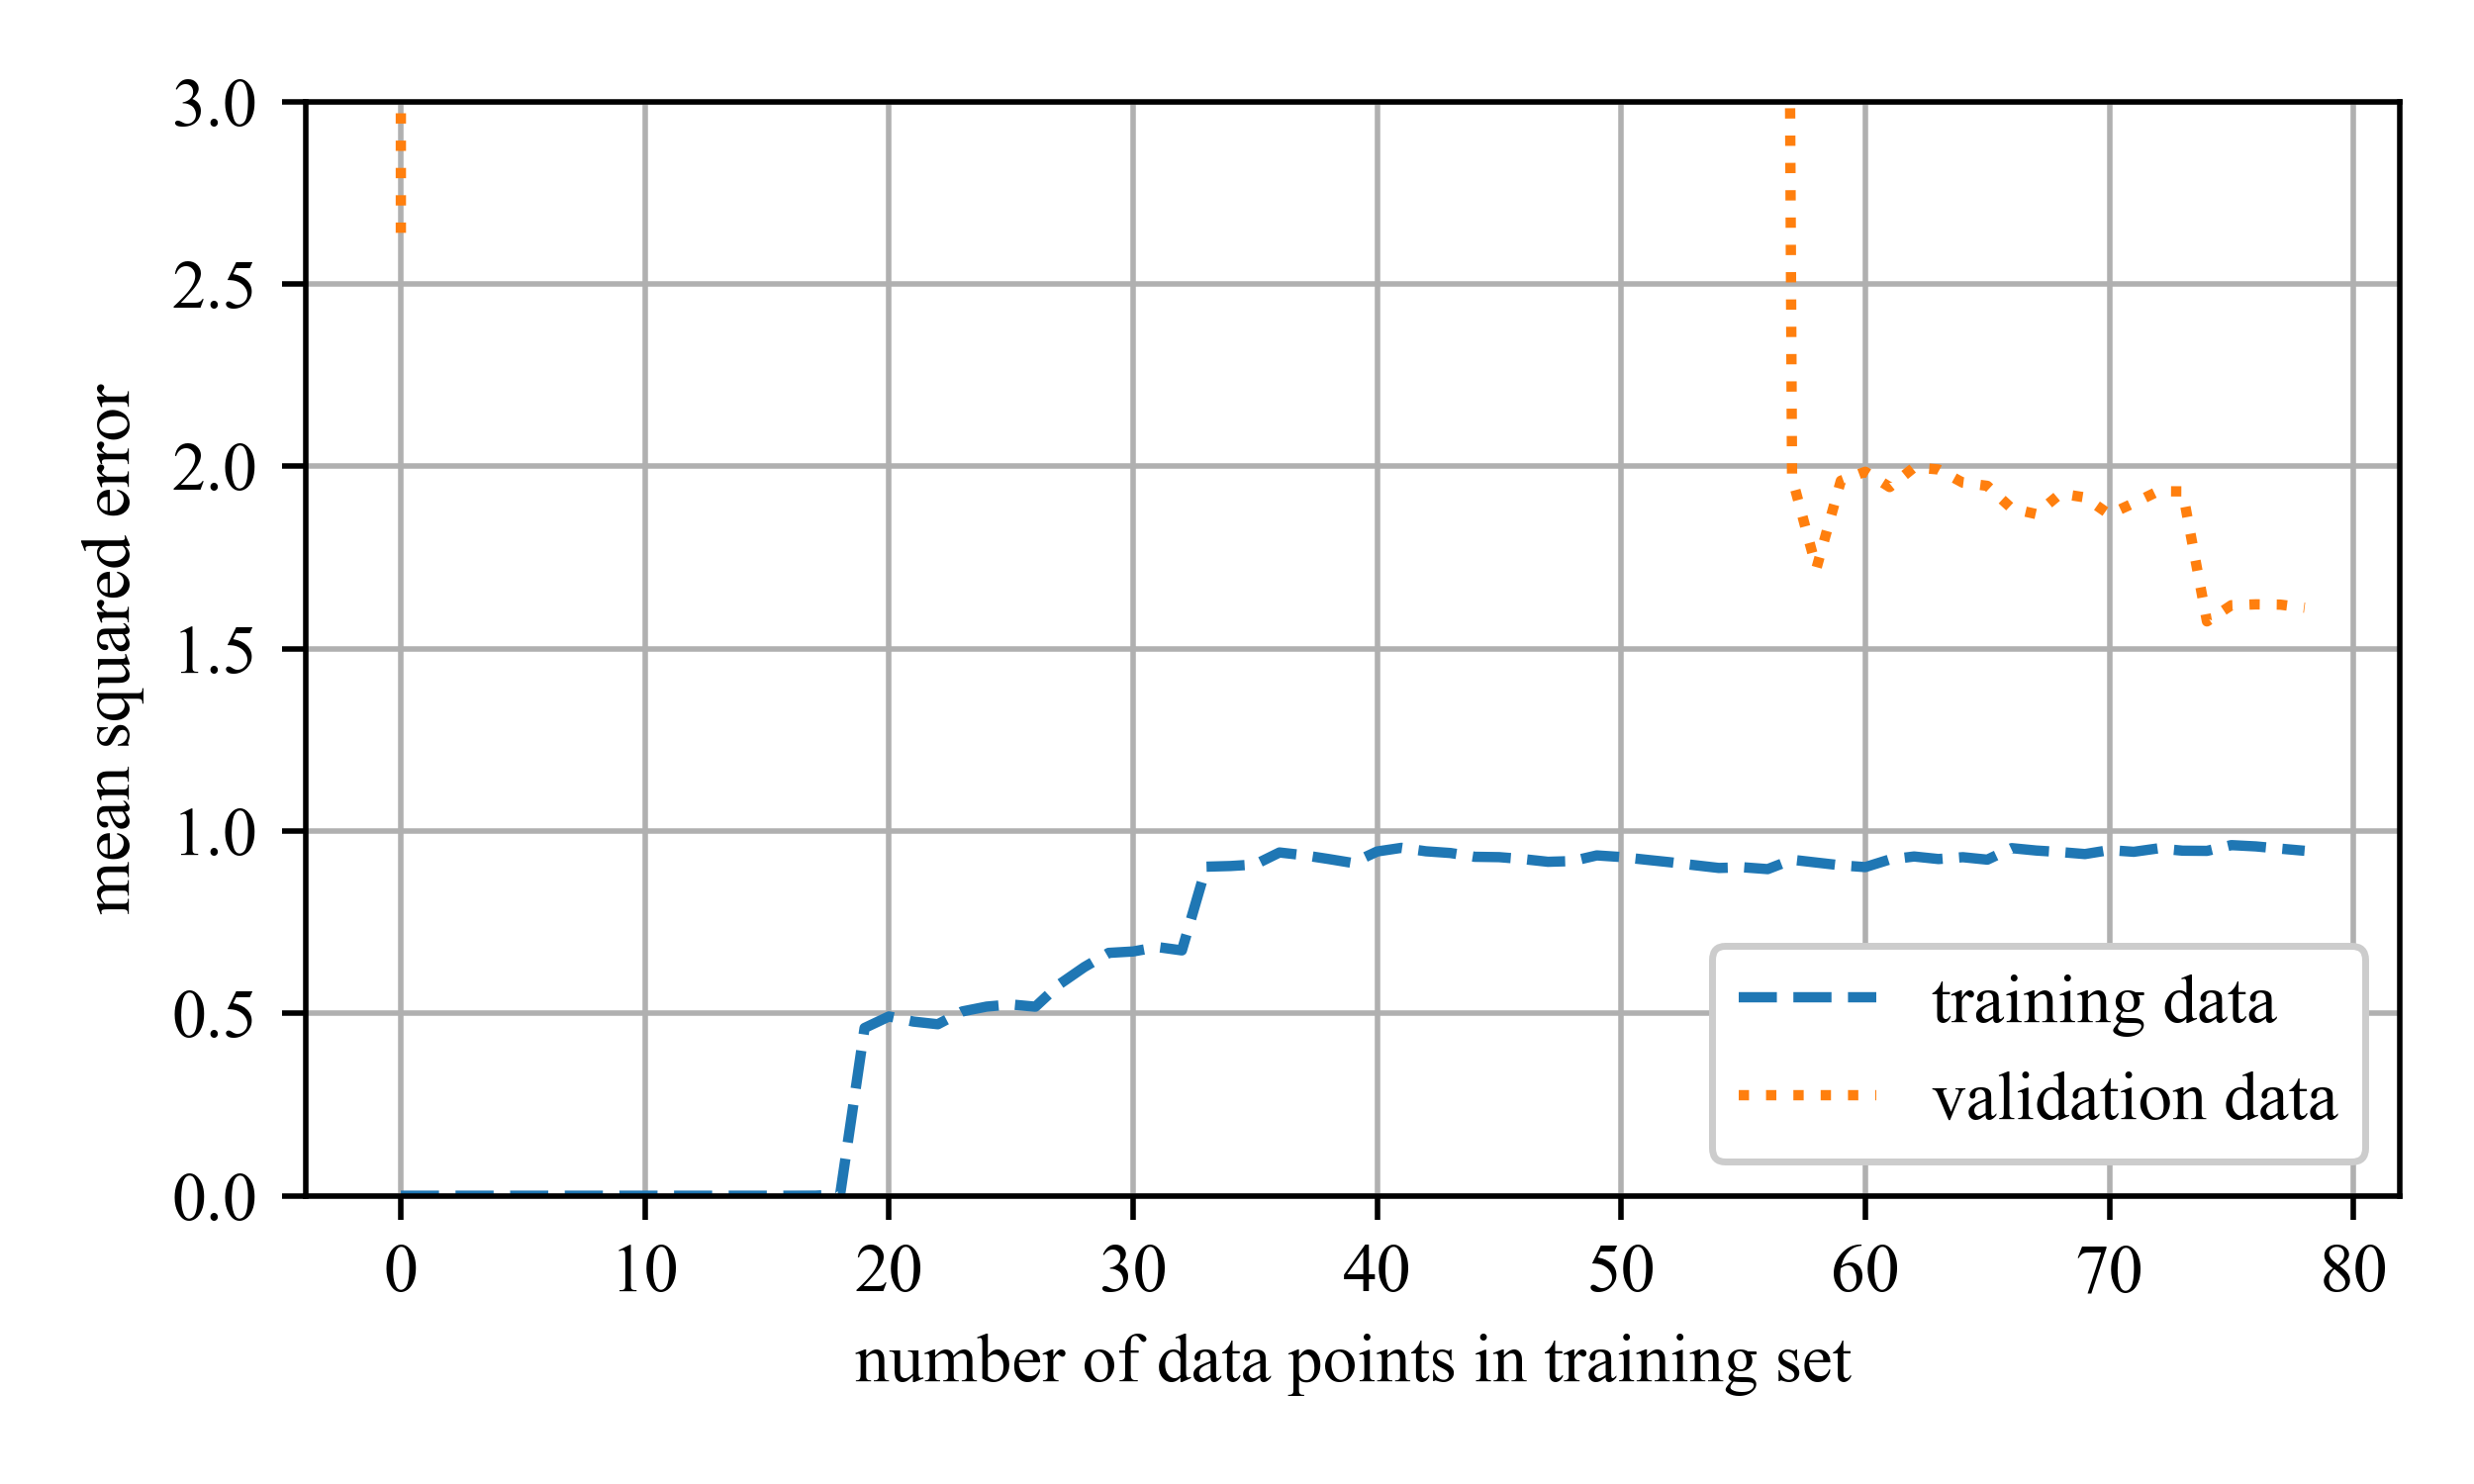
\includegraphics[]{../figures/overfitting_3.png}
    \caption{Learning curves for the overfitting polynomial model (degree=20) showing a significant gap between the curves, which indicates better performance on the training data than on the validation data.}
    \label{fig:overfitting_3}
\end{figure}

Inspection of the validation curve in figure~\ref{fig:overfitting_3}  tells a complementary story. With only a handful of training samples the model cannot generalize, so the validation error starts high. As more examples become available it learns progressively better patterns and the error falls. Eventually, though, the simple linear hypothesis is unable to capture the data's full complexity, causing the decline to flatten out; the validation curve plateaus at nearly the same level as the training curve. Their close proximity and uniformly large values are characteristic of an underfitting model.


Figure~\ref{fig:overfitting_3} displays the learning curves for a model fitted with a 20\textsuperscript{th}-degree polynomial. The overall shape resembles the curves seen earlier, yet two key differences stand out. First, the error on the training set is far lower than that achieved by the Linear Regression model, demonstrating the polynomial's extra flexibility. Second, a pronounced gap separates the training and validation curves, which means the model performs much better on the data it has already seen; this divergence is the hallmark of overfitting. Expanding the training set could reduce the gap, but without additional regularization the risk of overfitting would remain.


Next, let's apply the code using a 2\textsuperscript{nd} order polynomial, which accurately captures the essence of the data without underfitting or overfitting. These results are shown in Figure~\ref{fig:overfitting_4}. Here it can be seen that the training and validation curves again meet after converging, showing a well-fit model.

\begin{figure}[H]
    \centering
    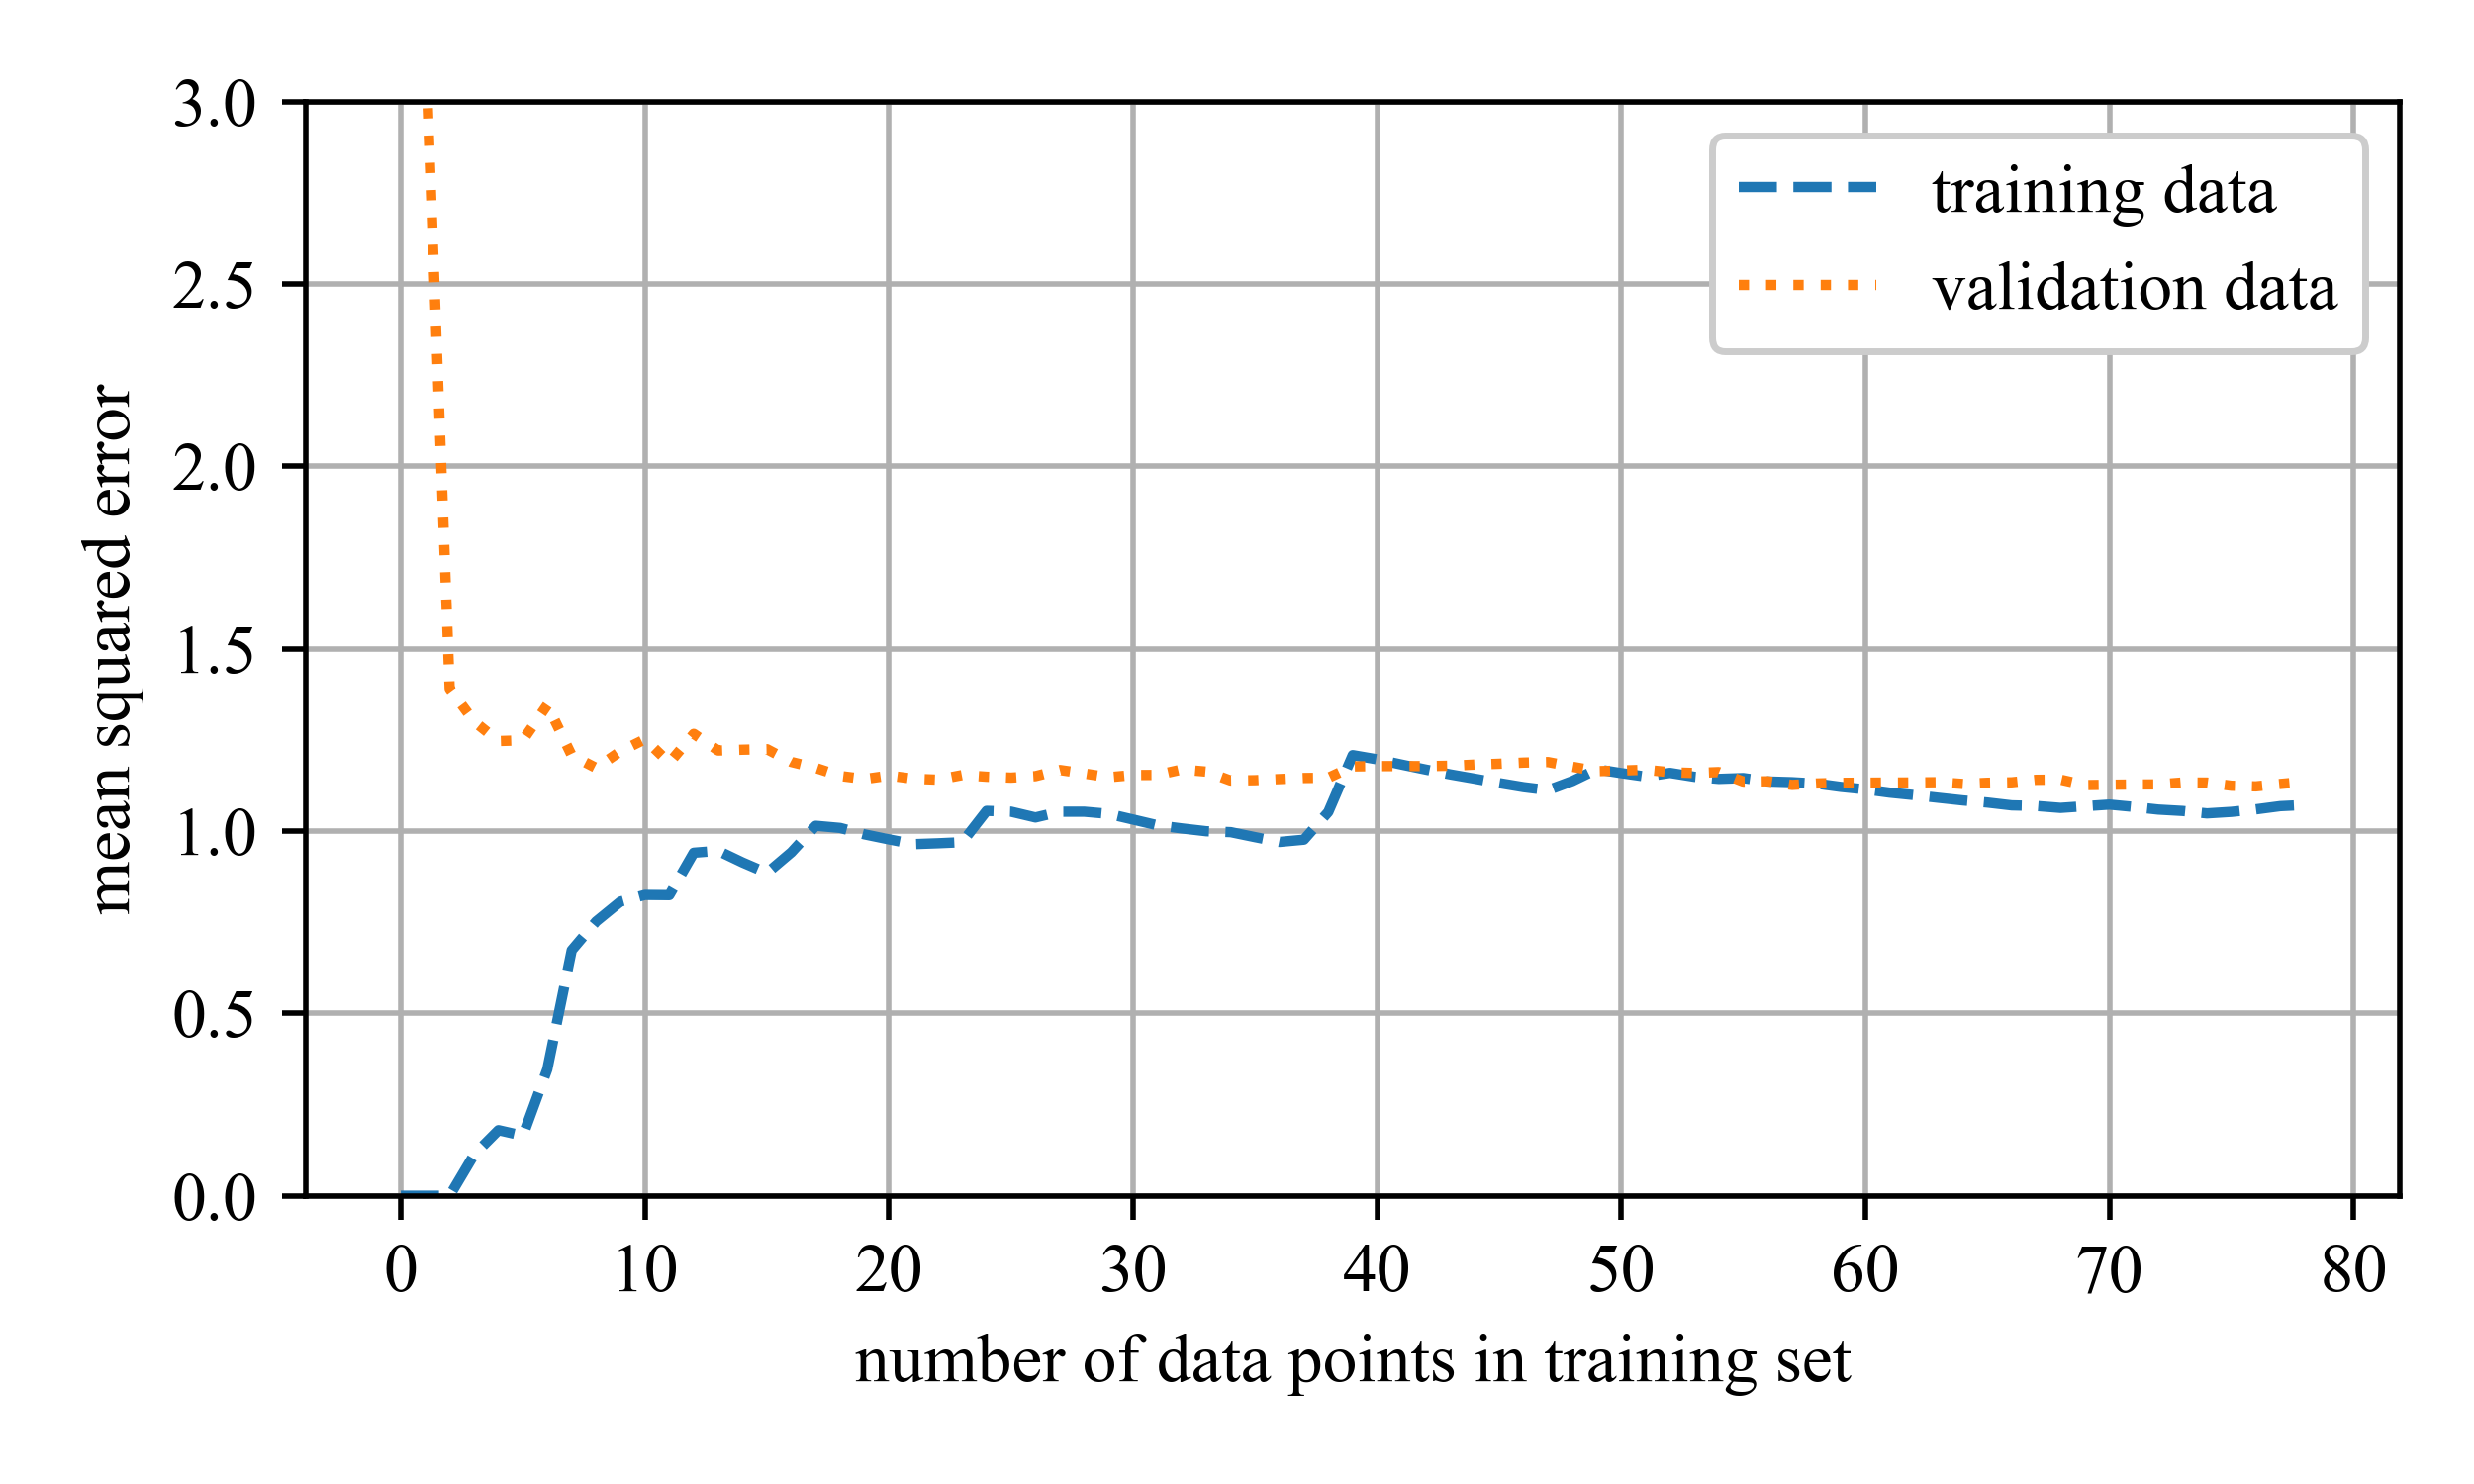
\includegraphics[]{../figures/overfitting_4.png}
    \caption{Learning curves for the optimal polynomial model (degree=2) showing well-aligned curves that plateau at a relatively low error level.}
    \label{fig:overfitting_4}
\end{figure}



\begin{example}
\textbf{Learning Curves}

\noindent This example compares learning curves for linear and polynomial regression models. By plotting training and validation errors as the training set grows, it illustrates how model complexity impacts bias and variance, and helps identify underfitting and overfitting behavior.
\end{example}




\subsection{Regularized Linear Models}
Overfitting is frequently curbed by regularizing the model, meaning you introduce constraints that reduce its effective degrees of freedom and make it harder to memories noise. In a polynomial setting you can achieve this simply by choosing a lower-degree polynomial, while in a linear model you typically add a penalty that discourages large coefficient values. This naturally raises the question: how is regularization expressed mathematically?


\subsubsection{Ridge Regression}

% \todo{Clarify the benefits of ridge regression and refine the description.}



Ridge Regression modifies Linear Regression by adding a regularization term to the cost function, which compels the learning algorithm to fit the data while keeping the model weights as small as possible. The updated cost-function is
\begin{equation}
J(\theta) = \text{MSE}(\theta) + \alpha \frac{1}{2} \sum_{i=1}^{n} \theta_i^2.
\label{eq:ridge_regression}
\end{equation}
The hyperparameter $\alpha$ dictates the degree of regularization. If $\alpha = 0$, Ridge Regression reduces to plain Linear Regression. If $\alpha$ is very high, the model weights are significantly shrunk, resulting in a nearly flat line through the mean of the data. Equation~\ref{eq:ridge_regression} outlines the cost function for Ridge Regression. The bias term $\theta_0$ is not regularized, as indicated by the summation starting from $i = 1$.

\begin{mdframed}[middlelinewidth=0.5mm]
\begin{center}
\bl{NOTE}
\end{center}
The regularization term is only included during the training phase. After training, the model's performance should be evaluated based on the unregularized performance measure.
\end{mdframed}

\begin{figure}[H]
    \centering
    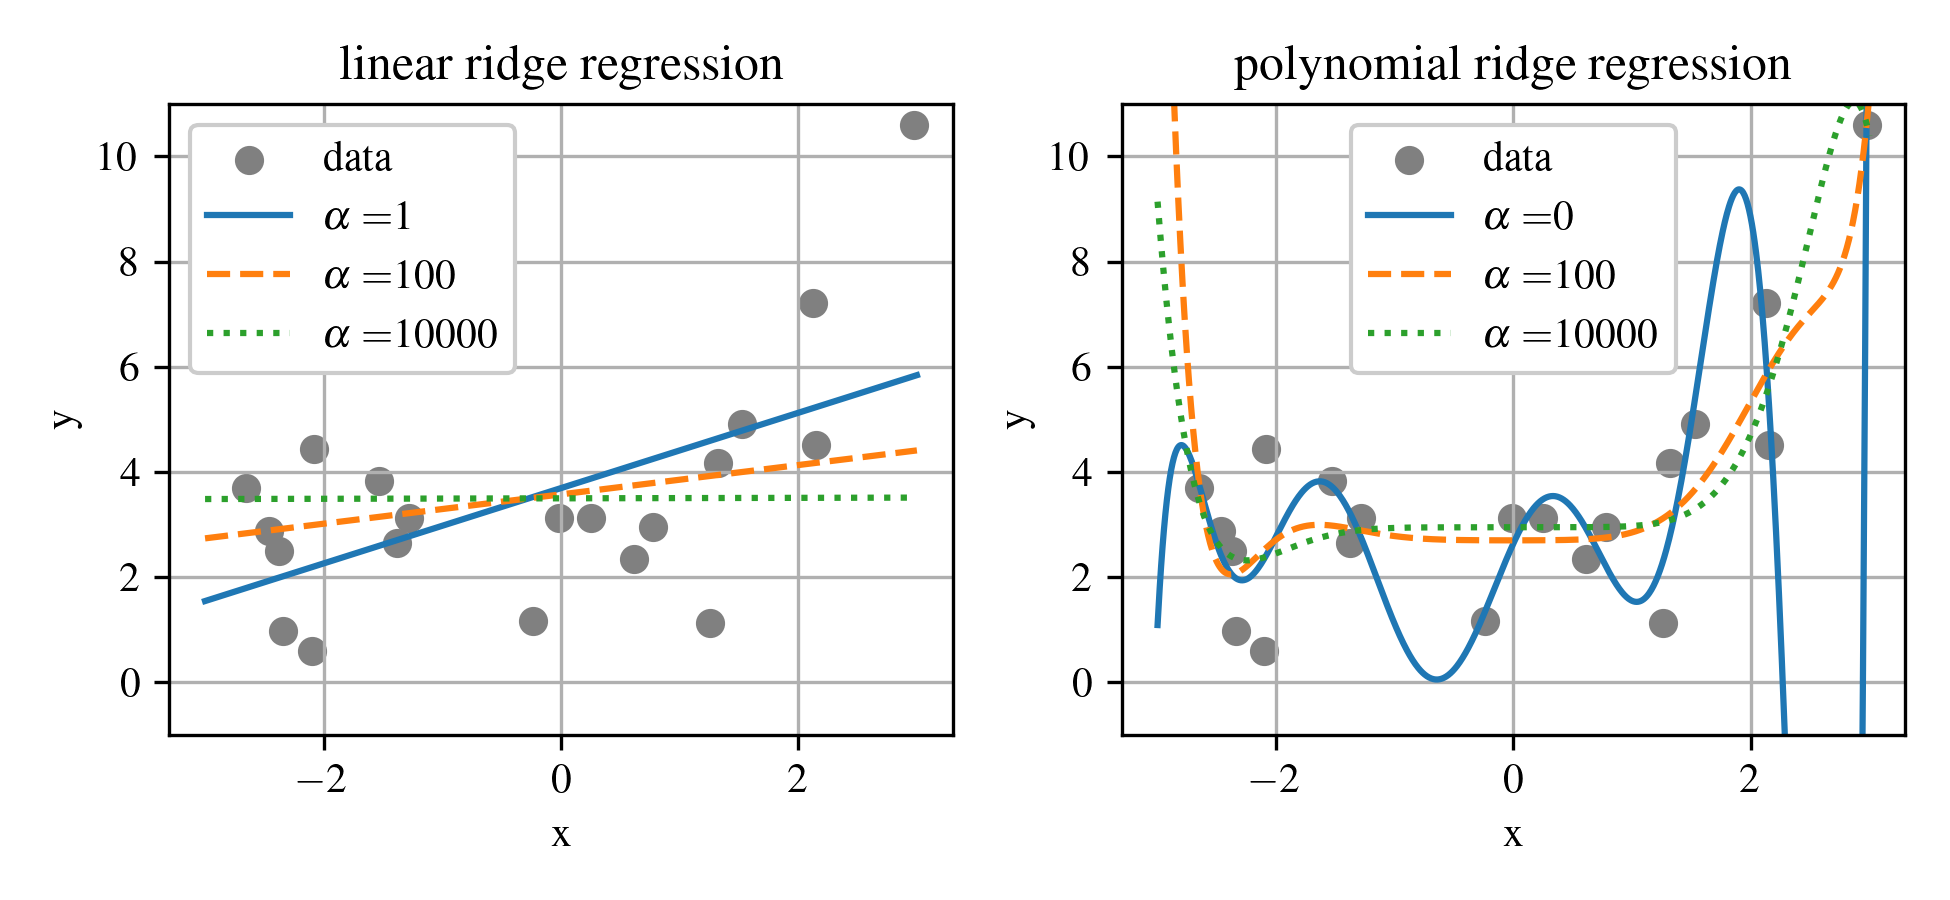
\includegraphics[width=6.5in]{../figures/ridge_regression.png}
    \caption{Visualization of Ridge Regression models with varying $\alpha$ values.}
    \label{fig:ridge_regression}
\end{figure}

Figure~\ref{fig:ridge_regression} illustrates various Ridge models trained on linear data, showcasing different $\alpha$ value. In Figure~\ref{fig:ridge_regression}(a), models are purely Ridge Regression, leading to linear predictions. In Figure~\ref{fig:ridge_regression}(b), the data undergoes Polynomial Regression with Ridge regularization. To do this, the data is first expanded using \texttt{PolynomialFeatures(degree=10)}, then scaled with \texttt{StandardScaler}, and finally, Ridge models are applied to these transformed features.


Increasing $\alpha$ results in flatter (i.e., more reasonable and less extreme) predictions, thereby reducing the model's variance but increasing its bias. Ridge Regression can be performed using a closed-form solution or through Gradient Descent, similar to Linear Regression. The pros and cons for each method mirror those discussed previously. The closed-form solution, an extension of the normal equation, is given by:
\begin{equation}
\hat{\theta} = (X^{\top} \cdot X + \alpha A)^{-1} \cdot X^{\top} \cdot y
\end{equation}
where $\alpha$ influences the regularization and $A$ is an $n \times n$ identity matrix with the top-left value replaced by 0 to exclude the bias term. When using Gradient Descent, the derivative of the cost function guides the adjustment toward optimal model parameters.

\begin{example}
\textbf{Ridge Regression}

\noindent This example demonstrates Ridge Regression as a regularized alternative to linear regression. A high-degree polynomial model is fit to noisy data using a pipeline with Ridge regularization, showing how the regularization term reduces overfitting and stabilizes the model.
\end{example}


%\subsubsection{Lasso Regression}
%
%\rd{Discuses other types of regularization.}
%
%
%
%\subsubsection{Elastic Net}
%
%\rd{Discuses other types of regularization.}

\subsection{Early Stopping}

An alternative approach to regularizing iterative learning methods 
(such as Gradient Descent) is to halt training as soon as the validation error hits its lowest point, a strategy known as early stopping. Figure~\ref{fig:early_stopping} illustrates a complex model, specifically a high-degree Polynomial Regression model, being refined through Batch Gradient Descent. Over the course of training, as epochs progress, the model's prediction error (RMSE) on both the training and validation sets decreases. However, after some time, the validation error ceases to decline and begins to increase, signaling that the model is beginning to overfit the training data. By implementing early stopping, training is terminated the moment the validation error reaches its minimum. Geoffrey Hinton praised this method stating, ``Early stopping (is) beautiful free lunch'' due to its simplicity \protect\footnotemark[1].

\footnotetext[1]{Pennington, Jeffrey, Richard Socher, and Christopher D. Manning. ``Glove: Global vectors for word representation.'' Proceedings of the 2014 conference on empirical methods in natural language processing (EMNLP). 2014.}


		\begin{figure}[H]
			\centering
			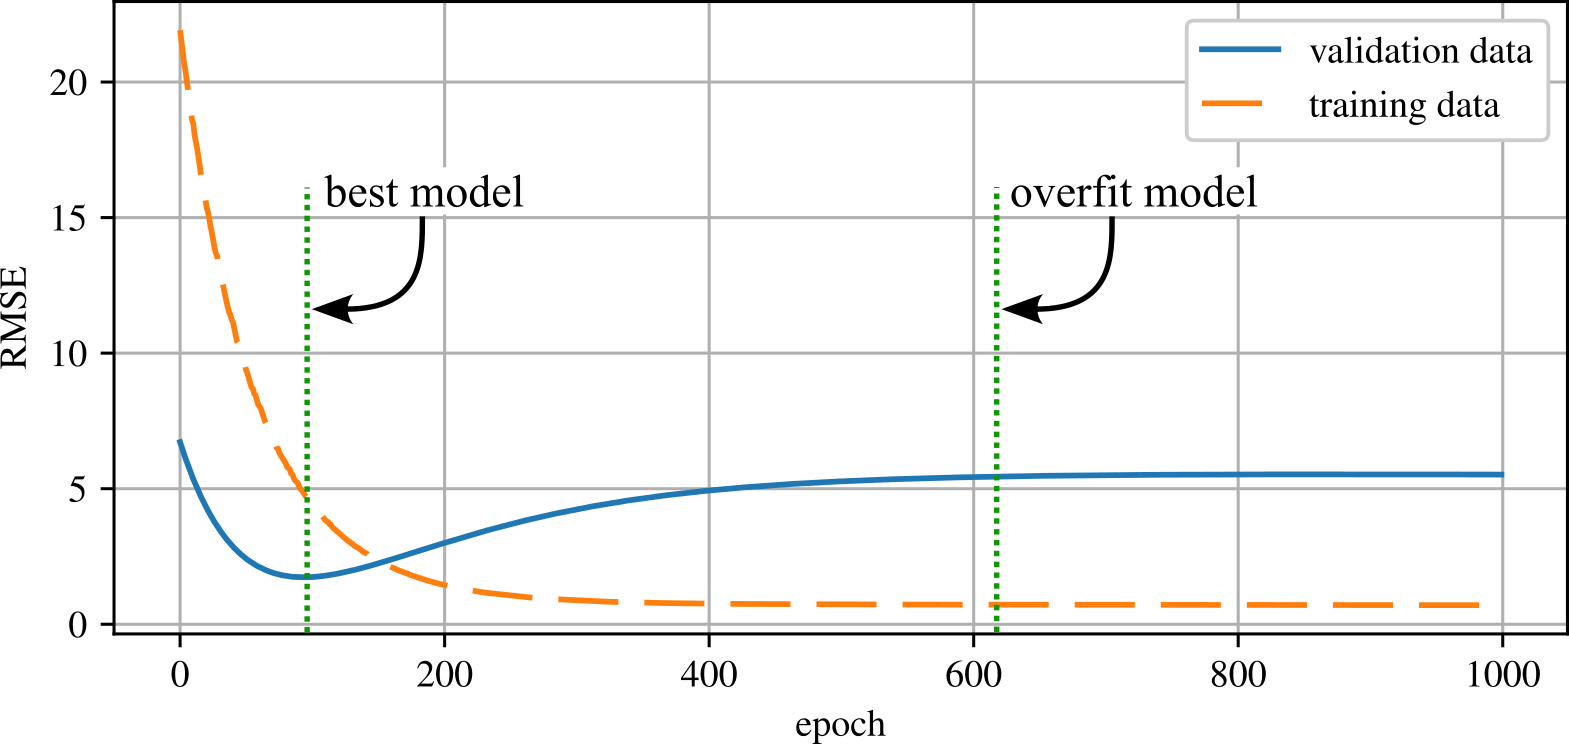
\includegraphics[width=6in]{../figures/early_stopping.png}
			\caption{An example showing how early stopping can result in a better model as it does not allow for the over-fitting of the training set.}
			\label{fig:early_stopping}
		\end{figure}


\begin{example}
\textbf{Early Stopping}

\noindent This example uses a high-degree polynomial model trained with stochastic gradient descent to demonstrate early stopping. By tracking training and validation errors across epochs, it highlights how halting training early can prevent overfitting and improve generalization.
\end{example}


\pagebreak
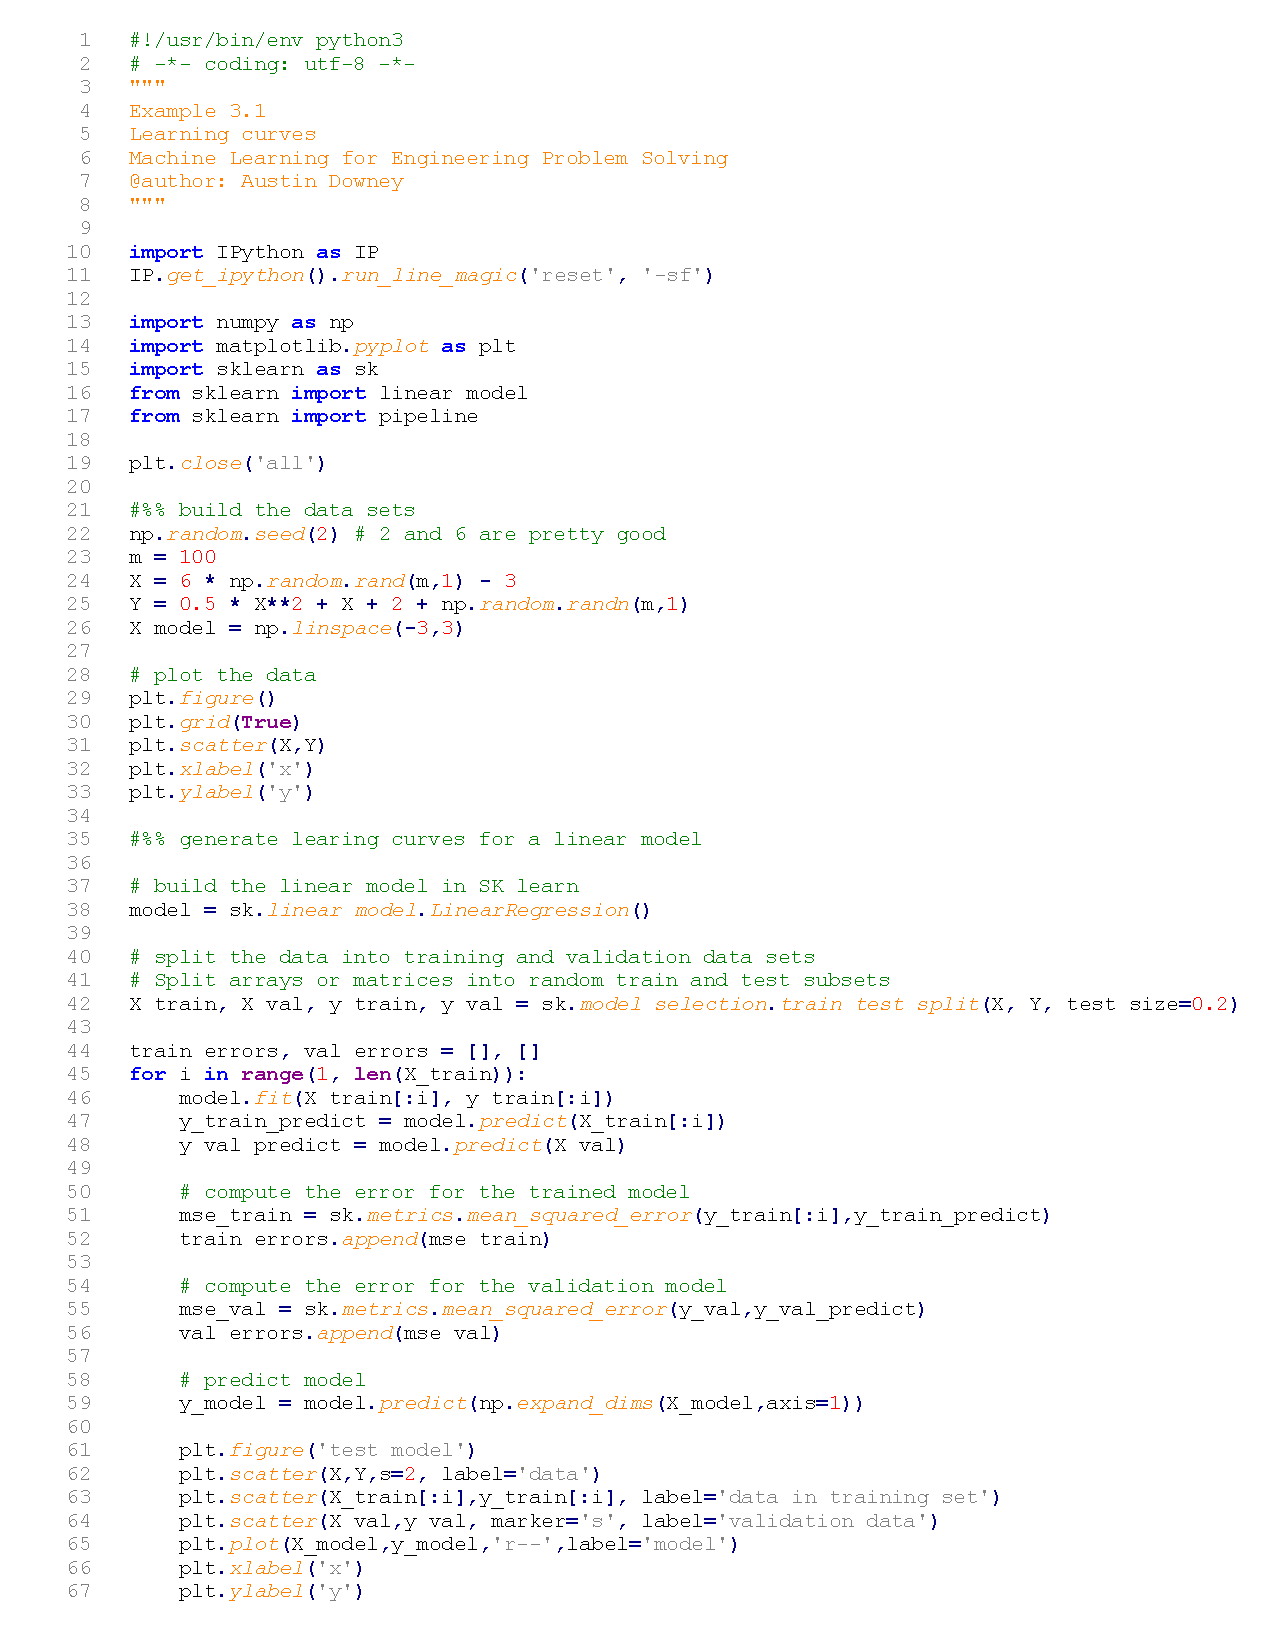
\includepdf[pages=1, width= 0.95\textwidth, pagecommand = {\subsection{Examples} 
\subsubsection*{Example 3.1}\vspace{0.5em}}]{../code/example_3.1_learning_curves.pdf}
\includepdf[pages=2, width= 0.95\textwidth, pagecommand = {\vspace{0.5em}}]{../code/example_3.1_learning_curves.pdf}

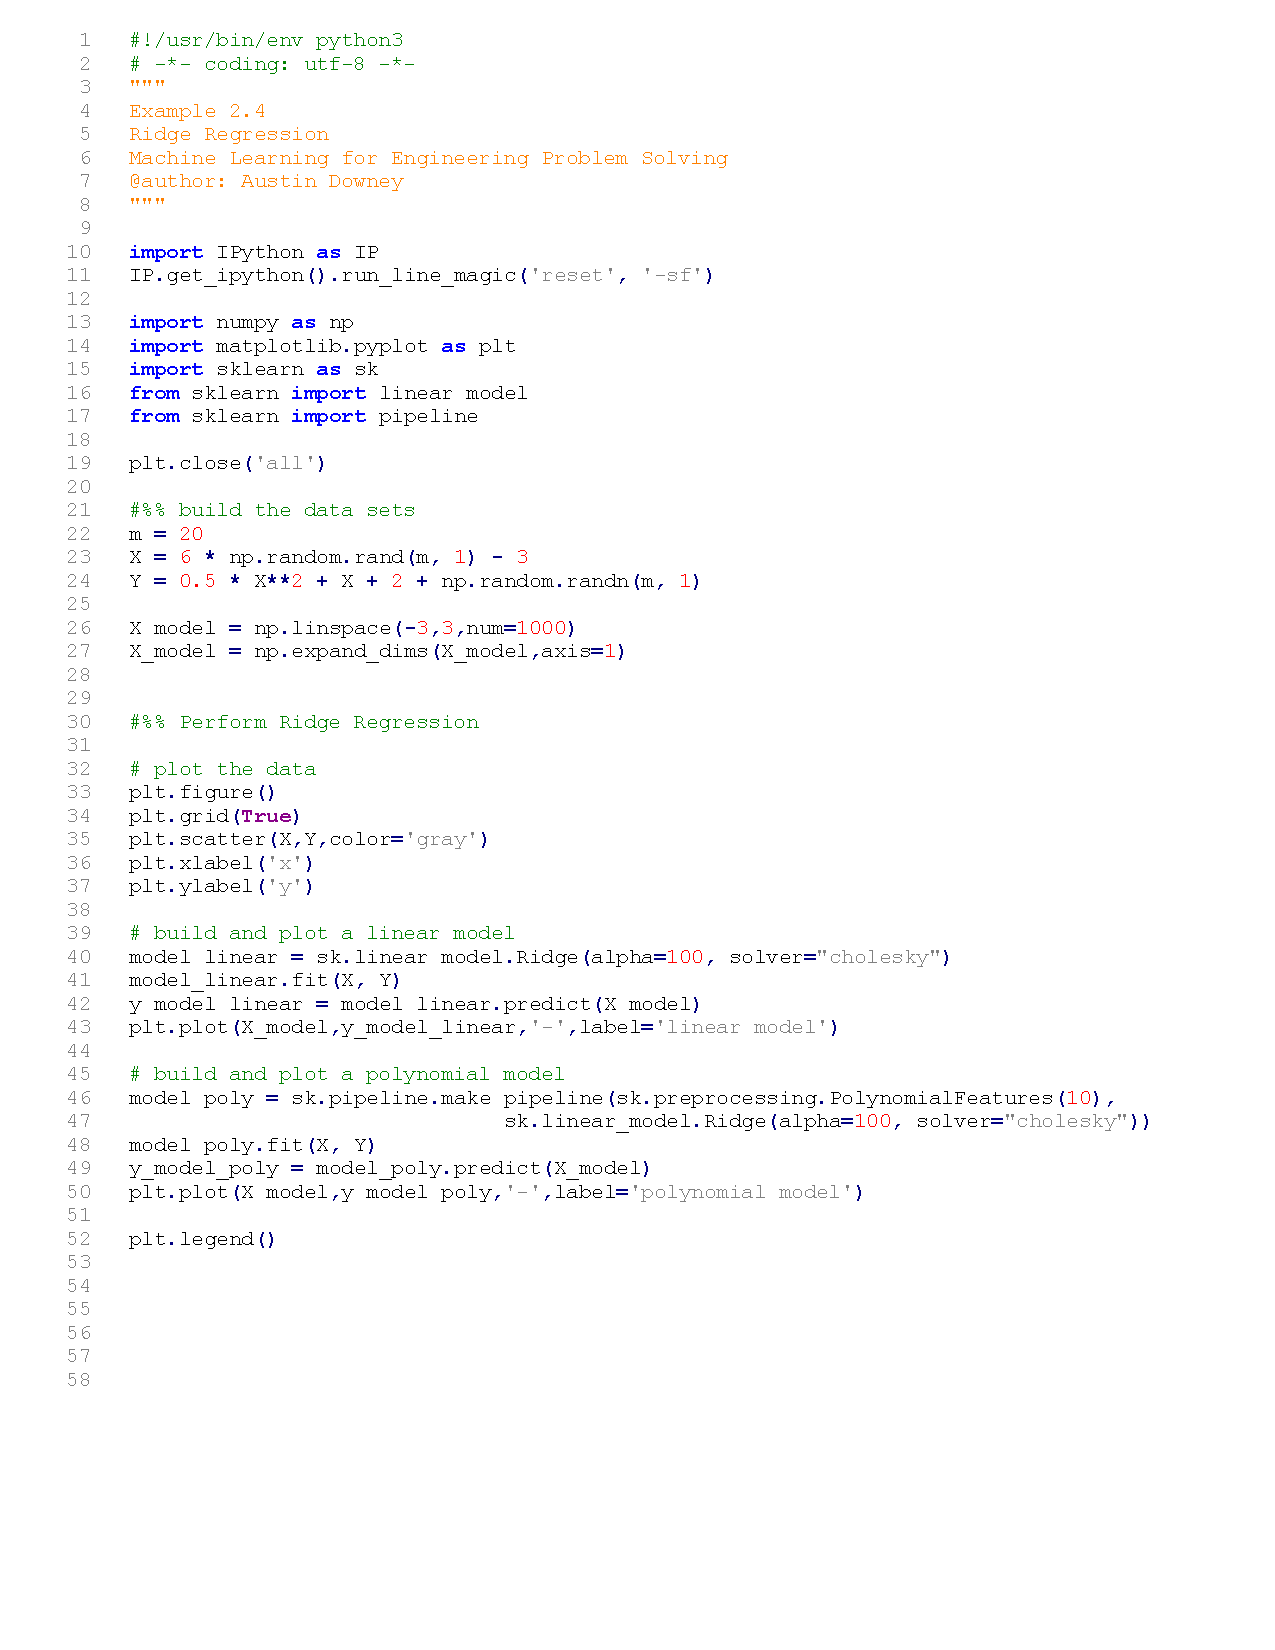
\includepdf[pages=-, width= 0.95\textwidth, pagecommand = {\subsubsection*{Example 3.2}\vspace{0.5em}}]{../code/example_3.2_ridge_regression.pdf}

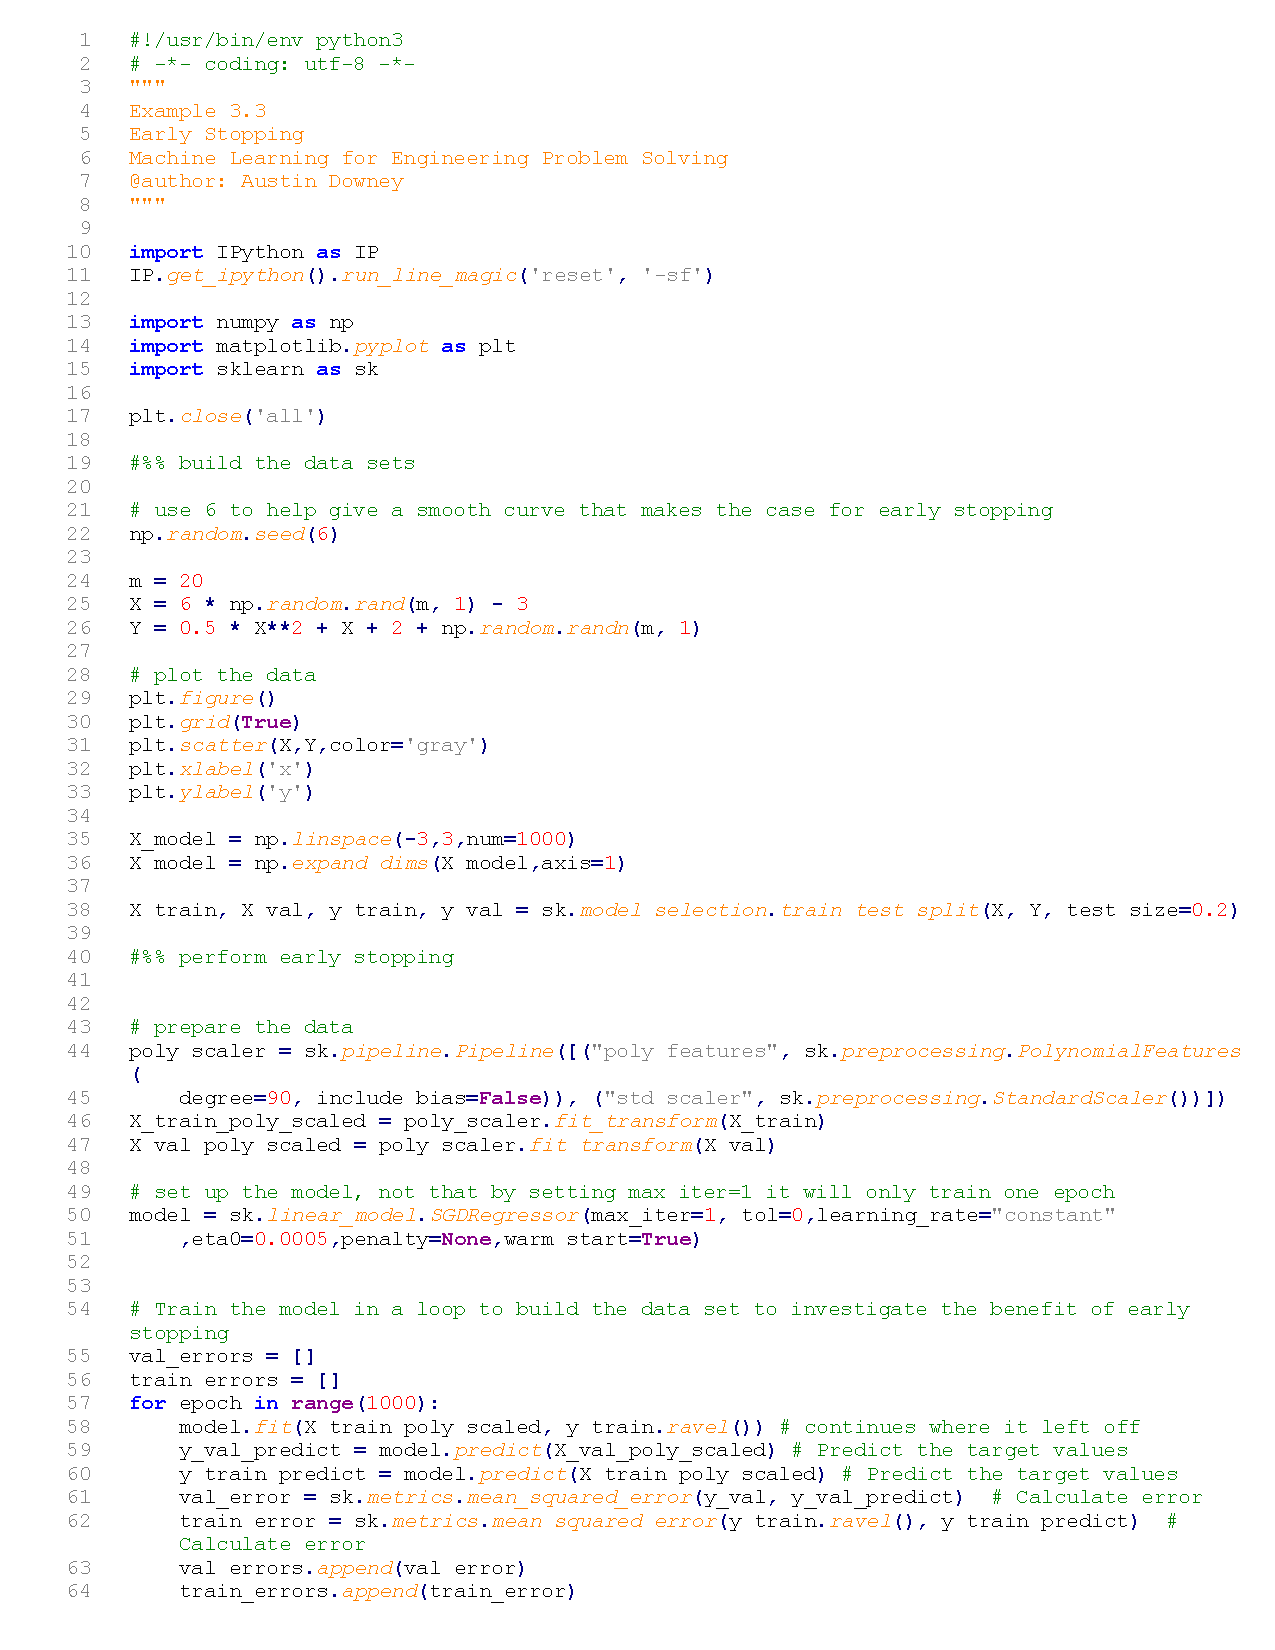
\includepdf[pages=1, width= 0.95\textwidth, pagecommand = {\subsubsection*{Example 3.3}\vspace{0.5em}}]{../code/example_3.3_early_stopping.pdf}
\includepdf[pages=2, width= 0.95\textwidth, pagecommand = {\vspace{0.5em}}]{../code/example_3.3_early_stopping.pdf}









\end{document}
